\section{Celda Sallen-Key}
El objetivo de esta secci\'on es la construcci\'on de dos filtros que cumplan con un conjunto de especificaciones,
empleando para el dise\~no en cascada la celda Sallen-Key. Para esto \'ultimo, es necesario primero realizar un an\'alisis ideal
y real de dicha celda para obtener ciertas conclusiones que faciliten el proceso de dise\~no e impongan restricciones sobre
las exigencias que se definan a cada etapa. Es importante aclarar que s\'olo se analizar\'a la celda pasabajos de Sallen-Key dado
que es la \'unica necesaria para la realizaci\'on de los filtros en cuesti\'on.

\subsection{Celda 2do Orden Sallen-Key: An\'alisis ideal}
En el siguiente an\'alisis se asume un comportamiento ideal del amplificador operacional, considerando una impedancia de entrada del mismo
$Z_{IN} \rightarrow \infty$, corrientes de entrada e impedancia de salida nulas, y finalmente una ganancia tambi\'en $A_{VOL} \rightarrow \infty$.

El an\'alisis ideal consiste en determinar la funci\'on transferencia y los par\'ametros caracter\'isticos para configurar la celda, as\'i como tambi\'en un an\'alisis de las sensibilidades relativas
respecto de los componentes a utilizar y un conjunto de estrategias propuestas para poder realizar el ajuste correcto de la celda. Por otro lado, es de inter\'es analizar las impedancias de entrada y salida de la celda,
ya que las mismas son las que permiten determinar hasta qu\'e punto es v\'alido asumir que en la conexi\'on en cascada no se produce una carga de una etapa con otra y efectivamente se puede aproximar $H(s) = H_1(s) \cdot H_2(s) \cdot ... \cdot H_n(s)$.

\begin{figure}[H]
    \centering
    \includegraphics[scale=0.45]{../EJ1/Recursos/circuito_sallen_key_pasabajos.png}
    \caption{Celda Sallen-Key para pasabajos}
    \label{circuito_sallen_key_pasabajos}
\end{figure}

\subsubsection{Funci\'on transferencia y par\'ametros}
Dentro del marco de los criterios expuestos anteriormente, para hallar la funci\'on transferencia se define el par\'ametro de ganancia de la celda $K$, y luego
se plantean un conjunto de ecuaciones empleando las leyes de Kirchhoff. Finalmente, el sistema se resuelve y se obtiene la funci\'on $H(s)$ de la cual se deducen par\'ametros
caracter\'isticos como $\omega_o$ y $Q$.

\begin{equation}
    K = 1 + \frac{R_B}{R_A}
    \label{eq:sallen_key_k}
\end{equation}

\begin{align*}
    & V_o = V_b \cdot K \\
    & V_b = V_a \cdot \frac{\frac{1}{s \cdot C_2}}{\frac{1}{s \cdot C_2} \cdot R_2} \\
    & \frac{V_i - V_a}{R_1} = \frac{V_a - V_o}{\frac{1}{s \cdot C_1}} + \frac{V_a - V_b}{R_2}
\end{align*}

\begin{equation}
    H(s) = \frac{K}{C_1 \cdot C_2 \cdot R_1 \cdot R_2 \cdot s^{2} + s \cdot \left[ C_2 \cdot (R_1 + R_2) + C_1 \cdot R_1 \cdot (1 - K) \right] + 1}
    \label{eq:sallen_key_h}
\end{equation}

\begin{equation}
    \omega_o = \frac{1}{\sqrt{C_1 \cdot C_2 \cdot R_1 \cdot R_2}}
    \label{eq:sallen_key_wo}
\end{equation}

\begin{equation}
    Q = \frac{\sqrt{C_1 \cdot C_2 \cdot R_1 \cdot R_2}}{C_2 \cdot (R_1 + R_2) + C_1 \cdot R_1 \cdot (1 - K)}
    \label{eq:sallen_key_q}
\end{equation}

A partir de estos resultados se puede observar que el par\'ametro definido $K$ corresponde a la ganancia de la banda de paso, o en continua. Por otro lado, es importante
se\~nalar la influencia de tal ganancia, entre otras variables, sobre el valor del factor de calidad $Q$ del circuito. Esto \'ultimo deber\'a ser tenido en cuenta en el an\'alisis de sensibilidades.

\paragraph{Estabilidad de la $H(s)$:} Si se toma la funci\'on transferencia ideal, y luego aplicando la teor\'ia de la transformada de Laplace, todo polo tal que $Re(polo) \geq 0$ har\'a que el sistema se vuelva inestable,
por tanto la respuesta transitoria no logr\'a nunca estabilizarse y ante cualquier cambio brusco de excitaci\'on el sistema nunca puede converger a un estado estable. Para evitar que esto suceda, se impone una restricci\'on sobre el t\'ermino lineal,
dado que controla la parte real del polo, y de ah\'i se obtiene que:

\begin{equation}
    K < 1 + \frac{C_2}{C_1} \cdot (1 + \frac{R_2}{R_1})
\end{equation}

De aqu\'i que la ganancia de una celda de este tipo nunca puede superar un determinado valor, impuesto por el propio dise\~no de la frecuencia de corte.

\subsubsection{Sensibilidades}
En el siguiente an\'alisis se emplea la definici\'on de sensibilidades relativas para cada una de las magnitudes o par\'ametros caracter\'isticos de la funci\'on transferencia. Esto es,
calcular $S^{y}_x = \frac{x_o}{y(x_o)} \cdot \frac{\delta y}{\delta x}$.

\begin{table}[H]
    \centering
    \begin{tabular}{c c c c c c}
        $R_A$ & $R_B$ & $R_1$ & $R_2$ & $C_1$ & $C_2$ \\
        \hline \\
        $0$ & $0$ & $\frac{-1}{2}$ & $\frac{-1}{2}$ & $\frac{-1}{2}$ & $\frac{-1}{2}$ \\
        \\
        \hline
    \end{tabular}
    \caption{Sensibilidades de $\omega_o$}
\end{table}

\begin{table}[H]
    \centering
    \begin{tabular}{c c c c c c}
        $R_A$ & $R_B$ & $R_1$ & $R_2$ & $C_1$ & $C_2$ \\
        \hline \\
        $\frac{1}{K} - 1$ & $1 - \frac{1}{K}$ & $0$ & $0$ & $0$ & $0$ \\
        \\
        \hline
    \end{tabular}
    \caption{Sensibilidades de $K$}
\end{table}

\begin{table}[H]
    \centering
    \begin{tabular}{c | c}
        \hline \\
        $K$ & $K \cdot Q \cdot \sqrt{\frac{C_1 \cdot R_1}{C_2 \cdot R_2}}$ \\
        \\ \hline \\
        $R_A$ & $-Q \cdot \frac{R_B}{R_A} \cdot \sqrt{\frac{R_1 \cdot C_1}{R_2 \cdot C_2}}$ \\
        \\ \hline \\
        $R_B$ & $Q \cdot \frac{R_B}{R_A} \cdot \sqrt{\frac{R_1 \cdot C_1}{R_2 \cdot C_2}}$ \\
        \\ \hline \\
        $R_1$ & $\frac{-1}{2} + Q \cdot \sqrt{\frac{C_2 \cdot R_2}{C_1 \cdot R_1}}$ \\
        \\ \hline \\
        $R_2$ & $\frac{1}{2} - Q \cdot \sqrt{\frac{C_2 \cdot R_2}{C_1 \cdot R_1}}$ \\
        \\ \hline \\
        $C_1$ & $\frac{-1}{2} + Q \cdot \left[ \sqrt{\frac{C_1 \cdot R_1}{C_2 \cdot R_2}} + \sqrt{\frac{C_1 \cdot R_2}{C_2 \cdot R_1}} \right]$ \\
        \\ \hline \\
        $C_2$ & $\frac{1}{2} - Q \cdot \left[ \sqrt{\frac{C_1 \cdot R_1}{C_2 \cdot R_2}} + \sqrt{\frac{C_1 \cdot R_2}{C_2 \cdot R_1}} \right]$ \\
        \\ \hline
    \end{tabular}
    \caption{Sensibilidades de $Q$}
\end{table}

\subsubsection{M\'etodos de ajuste}
En el proceso de dise\~no en cascada, para la composici\'on de cada una de las etapas se realiza una agrupaci\'on de ceros y polos acordes para la formaci\'on de una 
funci\'on transferencia que pueda ser implementada por alguna de las celdas existentes o disponibles, no obstante su implementaci\'on requiere de un proceso de ajuste para garantizar
el dise\~no menos sensible a variaciones por imperfecciones de los componentes o efectos par\'asitos de los mismos. En este apartado se proponen y analizan diferentes m\'etodos o enfoques de dise\~no, 
determinando sus beneficios al momento de ajustar los par\'ametros de la celda a la etapa deseada.

\paragraph{Dise\~no por componentes iguales:} Como estrategia de dise\~no para facilitar la elecci\'on de componentes ante los grados de libertad de los cuales se disponen,
se propone $R = R_1 = R_2$ y luego $C = C_1 = C_2$. De esta imposici\'on se simplifican las expresiones de los par\'ametros y de las sensibilidades, obteniendo:

\begin{equation}
    \omega_o = \frac{1}{R \cdot C}
    \label{eq:wo_ajuste_componentes_iguales}
\end{equation}

\begin{equation}
    Q = \frac{1}{3 - K}
    \label{eq:q_ajuste_componentes_iguales}
\end{equation}

\begin{table}[H]
    \centering
    \begin{tabular}{c | c}
        \hline \\
        $K$ & $\frac{K}{3 - K}$ \\
        \\ \hline \\
        $R_A$ & $-Q \cdot \frac{R_B}{R_A}$ \\
        \\ \hline \\
        $R_B$ & $Q \cdot \frac{R_B}{R_A}$ \\
        \\ \hline \\
        $R_1$ & $\frac{-1}{2} + Q$ \\
        \\ \hline \\
        $R_2$ & $\frac{1}{2} - Q$ \\
        \\ \hline \\
        $C_1$ & $\frac{-1}{2} + Q \cdot 2$ \\
        \\ \hline \\
        $C_2$ & $\frac{1}{2} - Q \cdot 2$ \\
        \\ \hline
    \end{tabular}
    \caption{Sensibilidades de $Q$}
\end{table}

Estos resultados revelan que si bien es m\'as simple la elecci\'on de componentes, el ajuste de la celda se vuelve m\'as complejo cuando la etapa requiere una selectividad alta,
provocando que ante variaciones de los componentes, para sistemas de selectividad muy alta, cambie el comportamiento del sistema dr\'asticamente. No obstante, este enfoque puede simplificar
el proceso de dise\~no en los casos donde se requiera un Q bajo.

\paragraph{Dise\~no por componentes proporcionales:} Como estrategia se impone que no haya ganancia de banda de paso en esta etapa, es decir que $K = 1$, y luego que los componentes sean proporcionales
entre s\'i, para lo cual se definen dos constantes de proporcionalidad tomando como referencia $R_2 = R \Rightarrow R_1 = m \cdot R$ y $C_2 = C \Rightarrow C_1 = n \cdot C$.

\begin{equation}
    \omega_o = \frac{1}{R \cdot C \cdot \sqrt{m \cdot n}}
    \label{eq:wo_ajuste_componentes_propocionales}
\end{equation}

\begin{equation}
    Q = \frac{\sqrt{m \cdot n}}{1 + m}
    \label{eq:q_ajuste_componentes_proporcionales}
\end{equation}


\begin{table}[H]
    \centering
    \begin{tabular}{c | c}
        \hline \\
        $K$ & $\frac{m \cdot n}{1 + m}$ \\
        \\ \hline \\
        $R_A$ & $\frac{m \cdot n}{1 + m} \cdot \frac{R_B}{R_A}$ \\
        \\ \hline \\
        $R_B$ & $- \frac{m \cdot n}{1 + m} \cdot \frac{R_B}{R_A}$ \\
        \\ \hline \\
        $R_1$ & $\frac{-1}{2} + \frac{1}{1 + m}$ \\
        \\ \hline \\
        $R_2$ & $\frac{1}{2} - \frac{1}{1 + m}$ \\
        \\ \hline \\
        $C_1$ & $\frac{-1}{2} + Q \cdot \left( \sqrt{\frac{m}{n}} + \sqrt{m \cdot n} \right)$ \\
        \\ \hline \\
        $C_1$ & $\frac{-1}{2} + Q \cdot \left( \sqrt{\frac{m}{n}} + \sqrt{m \cdot n} \right)$ \\
        \\ \hline
    \end{tabular}
    \caption{Sensibilidades de $Q$}
\end{table}

En primer lugar uno de los beneficios de esta estrategia es poder imponer restricciones adicionales sobre el dise\~no, como asignar valores a $m$ o a $n$ por separado. Esto \'ultimo permitir\'ia seg\'un
el caso minimizar la sensibilidad, suponiendo por ejemplo que $m = 1$, o en otro caso que $n = \frac{1}{2}$. Es importante aclarar que seg\'un el enfoque aplicado, los valores de referencia $R$ y $C$ son utilizados
para determinar el valor de la frecuencia de corte del filtro, no obstante las proporcionalidades permiten ajustar adem\'as la selectividad, con lo cual s\'olo uno de los dos criterios para minimizar la sensibilidad puede ser utilizado.
En segundo lugar, se puede observar que a diferencia de antes la estabilidad frente a variaciones de los valores nominales de componentes es mayor, no obstante esto implica una cota superior a la selectividad que puede garantizar esta celda,
para el caso donde $m = 1$ y luego, $Q = \frac{\sqrt{n}}{2}$.

En conclusi\'on, este enfoque de dise\~no permite seg\'un se tenga mayor probabilidad de variaciones en los capacitores o resistencias, ajustar las sensibilidades para minimizar el efecto de tales componentes,
y adem\'as definir los valores de forma m\'as simplificada. Adem\'as, al buscar que $K = 1$, se reduce el amplificador a un seguidor de tensi\'on o buffer, lo cual tiene sus ventajas al reducir los componentes necesitados
y aumentar el ancho de banda de tal etapa. Por otro lado, puede resultar que para valores grandes de Q este enfoque resulte en valores de capacitores muy grandes.

\paragraph{Dise\~no con atenuaci\'on:} Es posible que durante el uso de etapas se necesite uan determinada atenuaci\'on en la misma si se considera que la entrada puede ser de alta se\~nal, volviendose susceptible a saturar
y distorsionar. Esto \'ultimo, como se ver\'a posteriormente, afectar\'a directamente al rango din\'anmico de la celda dise\~nada. Por lo tanto, es deseable poder imponer una atenuaci\'on que mejore tales caracter\'isticas, pero en la
configuraci\'on propuesta no se puede conseguir un $K < 1$, salvo que se utilicen resistencias negativas con alg\'un circuito adicional pero eso agregar\'ia complejidad. Entonces, para solucionarlo se propone agregar una resistencia que produzca
una divisi\'on de tensi\'on, de forma tal que al aplicar el teorema de Thevenin, todo el an\'alisis previo es replicable asumiendo que la $R_1 = R_{TH} = R_{1_A} // R_{1_B}$.

\begin{figure}[H]
    \centering
    \includegraphics[scale=0.5]{../EJ1/Recursos/circuito_sallen_key_pasabajos_atenuado.png}
    \caption{Circuito Sallen-Key pasabajos con atenuaci\'on}
    \label{fig:sallen_key_pasabajos_atenuado}
\end{figure}

\begin{equation}
    A = \frac{R_{1_B}}{R_{1_A} + R_{1_B}}
\end{equation}

\begin{equation}
    H(s) = \frac{K \cdot A}{C_1 \cdot C_2 \cdot R_1 \cdot R_2 \cdot s^{2} + s \cdot \left[ C_2 \cdot (R_1 + R_2) + C_1 \cdot R_1 \cdot (1 - K) \right] + 1}
    \label{eq:sallen_key_h_atenuada}
\end{equation}

\subsubsection{Impedancia de entrada}
En la Fig. \ref{fig:circuito_sallen_key_impedancia_entrada_ideal} se puede observar que para calcular la impedancia de entrada se debe plantear un sistema de ecuaciones empleando 
las leyes de Kirchhoff correspondientes.

\begin{figure}[H]
    \centering
    \includegraphics[scale=0.5]{../EJ1/Recursos/circuito_sallen_key_impedancia.png}
    \caption{Circuito Sallen-Key pasabajos para c\'alculo de $Z_{IN}(s)$}
    \label{fig:circuito_sallen_key_impedancia_entrada_ideal}
\end{figure}

\begin{align*}
    & \frac{V_i - V_A}{R_1} = \frac{V_A}{R_2 + \frac{1}{s \cdot C_2}} + \frac{V_A - V_o}{\frac{1}{s \cdot C_2}} \\
    & V_o = V_A \cdot K \cdot \frac{\frac{1}{s \cdot C_2}}{R_2 + \frac{1}{s \cdot C_2}} \\
    & I_2 = \frac{V_A}{R_2 + \frac{1}{s \cdot C_2}} \\
    & I_1 = \frac{V_A - V_o}{\frac{1}{s \cdot C_1}}
\end{align*}

\begin{equation}
    Z_{IN}(s) = \frac{C_1 \cdot C_2 \cdot R_1 \cdot R_2 \cdot s^{2} + s \cdot \left[ C_2 \cdot (R_1 + R_2) + C_1 \cdot R_1 \cdot (1 - K) \right] + 1}{s \cdot \left[C_2 + C_1 \cdot (1 - K) \right] \cdot \left[ 1 + \frac{s \cdot C_1 \cdot C_2 \cdot R_2}{C_2 + C_1 \cdot (1 - K)} \right]}
    \label{eq:sallen_key_impedancia_entrada_ideal}
\end{equation}

A partir de la expresi\'on de la Ec. \ref{eq:sallen_key_impedancia_entrada_ideal}, en primer lugar se puede observar que la etapa como amplificador de transimpedancia es inestable y que para corriente continua la impedancia de entrada $Z_{IN} \rightarrow \infty$.
No obstante, es de inter\'es realizar un an\'alisis sobre esta expresi\'on que permita estimar de cierta forma una condici\'on de dise\~no para garantizar que la conexi\'on en cascada de la etapa es viable sin producir mayores desviaciones en la funci\'on transferencia total.

Se propone observar que la funci\'on $Z_{IN}(s)$ es de segundo orden, posee un polo en el origen y uno real, y luego dos ceros caracterizan un polinomio que es el mismo que el denominador de la funci\'on transferencia, lo cual tiene sentido
dado que caracteriza el comportamiento natural del sistema. A partir de esta observaci\'on se concluye que los ceros no influyen significativamente, sino que, asumiendo que el sistema se encuentra en todo caso cr\'iticamente amortiguado o subamortiguado y luego empleando las aproximaciones asint\'oticas
utilizadas en un diagrama de bode, se puede asumir que para las frecuencias de la banda de paso de este filtro, los ceros no tienen mayor influencia. As\'i, se reduce la complejidad del an\'alisis ya que cuando se vuelva apreciable el efecto que estas tienen, se estar\'a en la banda de transici\'on o de rechazo.
De esta forma, sea que el polo real se encuentra antes o despu\'es de dicha frecuencia de corte, para la banda de paso la impedancia de entrada es mon\'otona decreciente, con lo cual podemos estimar de manera aproximada que dentro de esta regi\'on de inter\'es el valor m\'inimo se encuentra sobre la frecuencia de corte,
con lo cual $Z_{IN_{min}} \approx Z_{IN}(s=j \cdot \omega_o)$. En la Fig. \ref{fig:grafico_zin_ideal_arbitraria} se observa un gr\'afico con valores arbitrarios para apreciar lo explicado.

\begin{figure}[H]
    \centering
    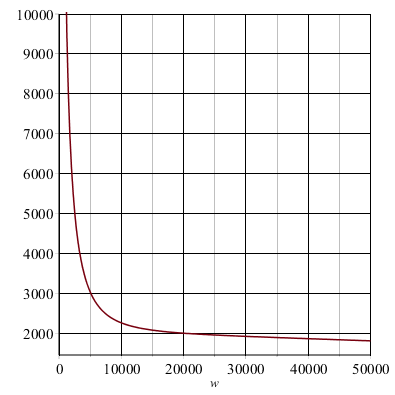
\includegraphics[scale=0.6]{../EJ1/Recursos/impedancia_entrada_arbitraria.png}
    \caption{Gr\'afico de $|Z_{IN}(j \cdot \omega)|$ con valores arbitrarios}
    \label{fig:grafico_zin_ideal_arbitraria}
\end{figure}

Entonces, reutilizando las expresiones presentadas y usando la definici\'on de la frecuencia de corte como se la encontr\'o en apartados anteriores, se llega a la siguiente expresi\'on de la impedancia de entrada
m\'inima en toda la banda de paso.

\begin{equation}
    Z_{IN_{min}} = \frac{C_2 \cdot (R_1 + R_2) + C_1 \cdot R_1 \cdot (1 - K)}{C_1 \cdot (1 - K) + C_2 + j \cdot \sqrt{\frac{C_1 \cdot C_2 \cdot R_2}{R_1}}}
\end{equation}

Puesto que se han propuesto m\'etodos de ajuste apropiados para la celda estudiada, se simplifica esta expresi\'on en el marco de tales enfoques, para obtener una expresi\'on
reducido en funci\'on de sus respectivos coeficientes o par\'ametros.

Para el dise\~no con componentes iguales:

\begin{equation}
    |Z_{IN_{min}}| = \frac{R \cdot |3 - K|}{\sqrt{K^{2} - 4 \cdot K + 5}}
    \label{eq:impedancia_minima_componentes_iguales}
\end{equation}

Para el dise\~no con componentes proporcionales:

\begin{equation}
    |Z_{IN_{min}}| = \frac{R \cdot (1 + m)}{\sqrt{1 + \frac{n}{m}}}
    \label{eq:impedancia_minima_componentes_proporcionales}
\end{equation}

\begin{figure}[H]
    \centering
    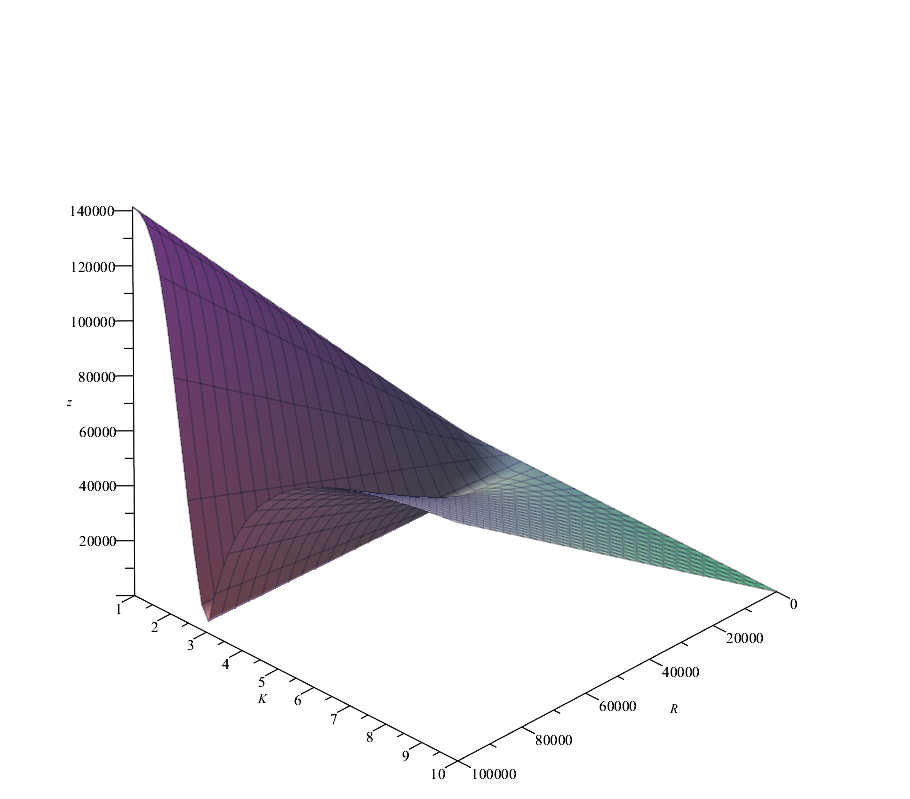
\includegraphics[scale=0.45]{../EJ1/Recursos/impedancia_entrada_componentes_iguales.png}
    \caption{Impedancia de entrada m\'inima con componentes iguales}
\end{figure}

\begin{figure}[H]
    \centering
    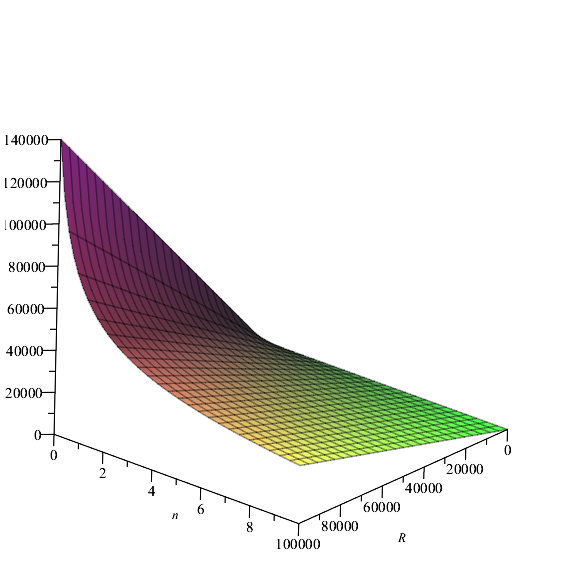
\includegraphics[scale=0.7]{../EJ1/Recursos/impedancia_entrada_componentes_proporcionales.png}
    \caption{Impedancia de entrada m\'inima con componentes proporcionales}
\end{figure}

\subsubsection{Impedancia de salida}
En el contexto de an\'alisis ideal, dado que la salida del circuito est\'a impuesta por un amplificador operacional con realimentaci\'on negativa,
luego la impedancia de salida tiende a ser nula. Es decir, $Z_O = 0$ siempre y cuando sea considerado un amplificador operacional ideal.

\subsection{Celda 2do Orden Sallen-Key: An\'alisis real}
A continuaci\'on se realiza un an\'alisis del comportamiento de la celda tomando consideraciones del amplificador operacional que no sean ideales,
no obstante el objetivo principal es estudiar de forma simplificada las desviaciones te\'oricas causadas por variaciones en su $A_{VOL}$, entre otros aspectos.
Es por esto que se sigue asumiendo una impedancia de entrada lo suficientemente grande en el amplificador para que las corrientes de entrada sean despreciables,
luego asumiendo que su ganancia de tensi\'on es grande, pero finita, y que var\'ia en funci\'on de la frecuencia, se hallan expresiones para la funci\'on transferencia,
la impedancia de entrada, de salida y algunas sensibilidades relacionadas con los nuevos par\'ametros reales tenidos en cuenta. 

\subsubsection{Funci\'on transferencia y par\'ametros}
Se reutiliza el an\'alisis ideal agregando como expresi\'on adicional para la resoluci\'on del sistema de ecuaciones,
que la relaci\'on impuesta por el amplificador operacional es en verdad $V_o = (V^{+} - V^{-}) \cdot A_{vol}$. Resolviendo
se puede obtener la nueva funci\'on de transferencia y sus par\'ametros.

\begin{equation*}
    H(s) = \frac{A_{vol} \cdot K}{A_{vol} + K} \cdot \frac{1}
    {s^{2} \cdot C_1 \cdot R_1 \cdot C_2 \cdot R_2
    + s \cdot \left[ \frac{(C_1 \cdot R_1 + C_2 \cdot R_1 + C_2 \cdot R_2) \cdot K}{A_{vol} + K} + A_{vol} \cdot \frac{C_2 \cdot (R_1 + R_2) + (1 - K) \cdot C_1 \cdot R_1}{A_{vol} + K} \right]
    +1}
    \label{eq:transferencia_sallen_key_real}
\end{equation*}

\begin{equation}
    \omega_o = \frac{1}{\sqrt{C_1 \cdot R_1 \cdot C_2 \cdot R_2}}
\end{equation}

\begin{equation}
    Q = \frac{(A_{vol} + K) \cdot \sqrt{C_1 \cdot R_1 \cdot C_2 \cdot R_2}}{K \cdot \left[ C_1 \cdot R_1 + C_2 \cdot (R_1 + R_2) \right] + A_{vol} \cdot \left[ C_2 \cdot (R_1 + R_2) + C_1 \cdot R_1 \cdot (1 - K) \right]}
\end{equation}

En primer lugar, es importante destacar que la frecuencia de corte de la celda se mantiene invariante frente a las variaciones del $A_{vol}$ seg\'un se de su valor en un circuito integrado o en otro. A los fines del an\'alisis buscado,
no es necesario, pero debe mencionarse que considerando adem\'as la disminuci\'on de la ganancia por la presencia del polo dominante como compensaci\'on para mejorar la estabilidad del amplificador, se incrementa en orden la funci\'on transferencia pero
el t\'ermino adicional tiene un efecto o una contribuci\'on que puede demostrarse no apreciable para las frecuencias que en relaci\'on al nuevo polo son bajas.
En segundo lugar, el valor de Q se ve significativamente afectado por la presencia del $A_{vol}$ por ello es necesario tener en cuenta cu\'an sensible es a variaciones por cambiar de un integrado a otro integrado,
para tener en cuenta durante los proceso de ajuste.

Por otro lado, en los casos donde sea necesario contrastar los resultados, se har\'a uso de esta \'ultima expresi\'on, analizandola con el polo dominante,
reemplazando por la expresi\'on de la Ec. \ref{eq:polo_dominante}, y luego reemplazando num\'ericamente para graficar.

\begin{equation}
    A_{vol} = \frac{GBP}{s + \omega_p}
    \label{eq:polo_dominante}
\end{equation}

\subsubsection{Sensibilidades}
Se resuelve algebraicamente la expresi\'on que define a la sensibilidad relativa, en este caso de Q, respecto del $A_{vol}$. Se hace de esta manera, ya que para todos los dem\'as par\'ametros
se realizo en el an\'alisis ideal, y si bien podr\'ia cambiar ligeramente se busca asumir para el dise\~no que el comportamiento ideal es suficiente para imponer tales restricciones.

\begin{equation}
    S^{Q}_{A_{vol}} = \frac{A_{vol}}{A_{vol} + K}
    - \frac{Q \cdot A_{vol}}{A_{vol} + K} \cdot \sqrt{C_1 \cdot C_2 \cdot R_1 \cdot R_2}
    \cdot \left[ C_2 \cdot (R_1 + R_2) + C_1 \cdot R_1 \cdot (1 - K) \right]
\end{equation}

A modo de verificaci\'on, puede observarse que si se hace tender a infinito la ganancia $A_{vol} \rightarrow \infty \Rightarrow S^{Q}_{A_{vol}} = 0$.
Lo cual denota que cuanto mayor sea su valor, luego m\'as invariante es el circuito ante sus variaciones.

\subsubsection{Impedancia de entrada}
Para estudiar la impedancia de entrada se reutilizan las expresiones y ecuaciones ya deducidas anteriormente, agregando
el siguiente sistema para encontrar la corriente total de entrada, y a partir de ello determinar la impedancia de entrada te\'orica.

\begin{align*}
    & I_{R_2} = \frac{V_a}{R_2 + \frac{1}{s \cdot C_2}} \\
    & I_{C_1} = \frac{V_a - V_o}{\frac{1}{s \cdot C_1}}
\end{align*}

\begin{equation}
    Z_{in}(s) = \frac{V_i}{I_{R_2} + I_{C_1}}
\end{equation}

\begin{equation}
    Z_{in}(s) = 
    \frac{\left( \frac{s}{\omega_o} \right)^{2} + s \cdot \frac{K \cdot (C_2 \cdot R_2 + C_2 \cdot R_1 + C_1 \cdot R_1) + A_{vol} \cdot (R_2 \cdot C_2 + C_2 \cdot R_1 + C_1 \cdot R_1 \cdot (1 - K))}{A_{vol} + K} + 1}
    {s \cdot \left[ s \cdot C_1 \cdot C_2 \cdot R_2 + \frac{(C_1 + C_2) \cdot K + A_{vol} \cdot (C_2 + C_1 \cdot(1 - K))}{A_{vol} + K} \right]}
\end{equation}

\subsubsection{Impedancia de salida}
En primer lugar, es importante remarcar que una de las principales funciones en realimentaci\'on negativa de un amplificador operacional ideal,
es la de mejorar la impedancia de salida disminuy\'endola en casos en donde dicha realimentaci\'on sea con salida de tensi\'on. En la pr\'actica este comportamiento
no es tan alejado, ya que se logra una impedancia de salida muy baja, no obstante el objetivo del an\'alisis es estudiar su respuesta en frecuencia para concluir
si en la conexi\'on en cascada, ante cambios bruscos en la excitaci\'on, existen inconvenientes.

\begin{figure}[H]
    \centering
    \includegraphics[scale=0.6]{../EJ1/Recursos/circuito_sallen_key_impedancia_salida.png}
    \caption{Circuito equivalente para impedancia de entrada}
    \label{fig:sallen_key_impedancia_salidas}
\end{figure}

Empleando las correspondientes leyes de Kirchhoff se logra llegar a un sistema de ecuaciones del cual se puede despejar la impedancia de salida, no obstante,
tal expresi\'on es demasiado extensa, y de su an\'alisis considerando los valores correspondientes al amplificador real usado, no pudo llegarse a una desviaci\'on
notoria respecto del resultado ideal. Esto se debi\'o a que el TL084 que se utiliz\'o, tiene entrada diferencial con JFET, con lo cual la $R_{ID}$ es tan grande que puede 
ser despreciada, luego $R_o$ es de aproximadamente $37 \Omega$, adem\'as luego la configuraci\'on empleada es de seguidor de tensi\'on por lo cual $R_B = 0\Omega$ y $R_A \rightarrow \infty$.
Aplicando estas simplificaciones al desarrollo, se obtiene la Ec. \ref{eq:impedancia_salida_simplificada}.

\begin{equation}
    Z_o(s) = \frac{R_o}{A_{vol} + 1} \cdot
    \frac{\left( \frac{s}{\omega_o} \right)^{2} + s \cdot (R_1 \cdot C_1 + R_1 \cdot C_2 + C_2 \cdot R_2) + 1}
    {\left( \frac{s}{\omega_o} \right)^{2} \cdot \left[ 1 + \frac{\frac{R_o}{R_1 // R_2}}{A_{vol} + 1} \right] + s \cdot \left[ C_2 \cdot (R_1 + R_2) + \frac{C_1 \cdot (R_1 + R_o)}{A_{vol} + 1} \right] + 1}
    \label{eq:impedancia_salida_simplificada}
\end{equation}

Es de inter\'es observar que, en primer lugar si se cumple que la ganancia es muy elevada, luego la $Z_o \approx 0$. En segundo lugar,
nuevamente el numerador tiene la misma forma que el denominador de la $H(s)$ y con ello las mismas implicancias que lo que se mencion\'o para la impedancia de entrada.

\subsubsection{Restricciones reales sobre impedancias}
El dise\~no de un filtro mediante la separaci\'on del sistema total en sistemas de segundo o primer orden, es en primer lugar algo que se busca para reducir la sensibilidad
de los par\'ametros del filtro frente a los valores de componentes empleados. En este proceso de separaci\'on, se busca la interconexi\'on de dichas etapas o celdas para lo cual
es necesario que se cumpla como condici\'on que una etapa o celda no cargue a la anterior para poder buscar que el sistema total sea descrito por el producto de las funciones transferencia
de las etapas.

\begin{figure}[H]
    \centering
    \includegraphics[scale=0.65]{../EJ1/Recursos/celda_representacion.png}
    \caption{Representaci\'on de una celda simplificada}
    \label{fig:celda_representacion}
\end{figure}

En la Fig. \ref{fig:celda_representacion} se puede observar una simplificaci\'on del modelo de una celda,
donde en particular es de inter\'es contemplar que para esta modelizaci\'on, la interconexi\'on de dos etapas $H_1(s)$ y $H_2(s)$
implica un t\'ermino adicional resultante del divisor entre sus resistencias de salida y entrada respectivamente.

\begin{equation}
    H(s) = H_1(s) \cdot H_2(s) \cdot \frac{R_{i_2}}{R_{i_2} + R_{o_1}}
\end{equation}

Es de gran importancia para garantizar el comportamiento esperado del filtro, que $R_{i_2}$ sea mucho m\'as grande que $R_{o_1}$, y as\'i
lograr establecer que $H(s) \approx H_1(s) \cdot H_2(s)$.

\subsubsection{Rango din\'amico}

\subsection{Celda 1er Orden pasabajos: An\'alisis ideal}
En el dise\~no de los filtros, en los casos donde es necesario un orden de transferencia impar, se requiere el uso de celdas de primer orden.
Particularmente en este caso se hace uso de un circuito RC simple con un amplificador operacional de seguidor de tensi\'on o buffer para adaptar las impedancias en la conexi\'on en cascada,
tal configuraci\'on se puede apreciar en la Fig. \ref{fig:circuito_pasabajos_primer_orden}.

\begin{figure}[H]
    \centering
        \includegraphics[scale=0.7]{../EJ1/Recursos/circuito_celda_primer_orden.png}
    \caption{Circuito 1er Orden Pasabajos}
    \label{fig:circuito_pasabajos_primer_orden}
\end{figure}

\subsubsection{Funci\'on transferencia}
Se puede calcular la funci\'on de transferencia considerando el amplificador operacional de forma ideal con su configuraci\'on de buffer,
luego la transferencia se puede reducir a un simple divisor resistivo de tensi\'on, como se muestra en la Ec. \ref{eq:funcion_transferencia_ideal_primer_orden}.

\begin{equation}
    H(s) = \frac{\frac{1}{s \cdot C}}{R + \frac{1}{s \cdot C}} = \frac{1}{1 + s \cdot C \cdot R}
    \label{eq:funcion_transferencia_ideal_primer_orden}
\end{equation}

Entonces, se puede ajustar sencillamente el circuito para ubicar el polo de primer orden necesario en la frecuencia correspondiente a $\omega_o = \frac{1}{R \cdot C}$.

\subsubsection{Impedancia de entrada}
Asumiendo condiciones de idealidad, como el amplificador operacional tiene una impedancia de entrada tal que $Z_{IN} \rightarrow \infty$, luego la corriente de entrada del mismo es nula
con lo cual la impedancia de entrada vista por el generador de informaci\'on se simplifica a la forme mostrada en Ec. \ref{eq:impedancia_entrada_primer_orden}.

\begin{equation}
    Z_{in}(s) = \frac{1}{s \cdot C} + R = \frac{s \cdot C \cdot R + 1}{s \cdot C}
    \label{eq:impedancia_entrada_primer_orden}
\end{equation}

La principal conclusi\'on de esto, es que para todo el rango de frecuencias se puede aproximar que la impedancia de entrada m\'inima es cuando la frecuencia es tal que el capacitor
tiene una reactancia nula, por ende la resistencia define el m\'inimo valor de impedancia del circuito. Ergo, $Z_{in_{min}} = R$. Lo cual deber\'a ser tenido en cuenta durante la conexi\'on
en cascada para poder asegurar que las etapas no se carguen entre s\'i.

\subsection{Dise\~no de un filtro con Legendre}
Entre las funciones de aproximaci\'on disponibles para el dise\~no de filtros, se pueden utilizar los polinomios de Legendre de los cuales
mediante procesos de c\'alculo se obtienen polinomios asociados que permiten construir una aproximaci\'on cuyas beneficios m\'as destacables son la m\'axima pendiente
de cambio en la frecuencia de banda de paso normalizada y una buena estabilidad del mismo.

\begin{equation}
    |H(j \cdot \omega_N)|^{2} = \frac{1}{1 + \xi^{2} \cdot L_n(\omega_N{2})}
\end{equation}

\subsubsection{Especificaciones y funci\'on aproximaci\'on}
Se desea dise\~nar un filtro pasabajos implementado con una funci\'on de Legendre para altas se\~nales que cumpla con las especificaciones
ilustradas en la Tabla \ref{table:especificaciones_legendre}.

\begin{table}[H]
    \centering
    \begin{tabular}{c | c}
        \hline \\
        Orden & $5$ \\
        \\ \hline \\
        $f_p$ & $27kHz$ \\
        \\ \hline \\
        $A_p$ & $3 dB$ \\
        \\ \hline \\
        $|Z_{IN}(f)|$ & $\geq 50k \Omega$ \\ 
        \\ \hline
    \end{tabular}
    \caption{Especificaciones de filtro con aproximaci\'on Legendre}
    \label{table:especificaciones_legendre}
\end{table}

A partir de las especificaciones dadas se obtiene el polinomio de Legendre de orden 5, y utilizando las ecuaciones correspondientes se llega a la funci\'on aproximaci\'on, es decir, la funci\'on
transferencia normalizada para la frecuencia unitaria que cumple con lo impuesto anteriormente. Luego se realiza una transformaci\'on de frecuencia para correr el filtro normalizado a la frecuencia deseada,
finalmente se obtiene la funci\'on a implementar con sus polos correspondientes, realizando un ajuste para la ganancia unitaria de la banda de paso si fuera necesario.

Los siguientes polos de la funci\'on aproximaci\'on fueron encontrados tomando un margen respecto de la plantilla consignada para conseguir mayor libertad en las desviaciones pr\'acticas por efectos par\'asitos de componentes.

\begin{table}[H]
    \centering
    \begin{tabular}{c | c}
        Polo & Ubicaci\'on \\
        \hline \\
        Complejo conjugado & $f_o = 28.371kHz$ y $Q = 2.88$ \\
        Complejo conjugado & $f_o = 21.313kHz$ y $Q = 0.84$\\
        Simple & $f_o = 15.527kHz$\\
        \\ \hline
    \end{tabular}
    \caption{Polos desnomarlizados de la $H(s)$}
\end{table}

\subsubsection{Dise\~no de etapas}
Para dise\~nar este filtro partiendo de los polos obtenidos de la aproximaci\'on de Legendre, se los separa en tres etapas. En primer lugar, es necesario tener en cuenta que como la se\~nal de entrada
es de amplitud grande seg\'un lo especificado, entonces es necesario ordenar la conexi\'on en cascada de las etapas de un menor a un mayor Q, para prevenir que en los sobrepicos de las frecuencias de corte
se produzca la saturaci\'on de las primeras etapas. Por otro lado, es necesario tener en cuenta que la etapa de entrada debe cumplir con lo consignado para la impedancia de entrada,
y entre s\'i las etapas deben estar correctamente balanceadas para no cargarse entre s\'i, con lo cual como idealmente la impedancia de salida de los amplificadores es nula, luego basta con tener una impedancia de entrada
relativamente grande para garantizar un correcto acoplamiento.

\paragraph{$1^{\circ}$ etapa:} Se dise\~na una etapa de filtro pasabajo con los par\'ametros $\omega_o = 2 \pi \cdot 15.527 kHz$. En primer lugar, como se desea que el filtro en general tenga una impedancia de entrada $\geq 50k \Omega$, entonces
esa misma restricci\'on se impone sobre $R$. Luego iterando sobre valores comerciales se encuentra con menos desviaci\'on nominal, donde $R = 100k \Omega$ y $100pF$. Si bien es un valor sensible para realizar mediciones, deber\'a ser tenido en cuenta
a la hora de escoger la punta de medici\'on, y contemplado al momento de observar los resultados siempre y cuando se mida sobre el capacitor.

\begin{figure}[H]
    \centering
    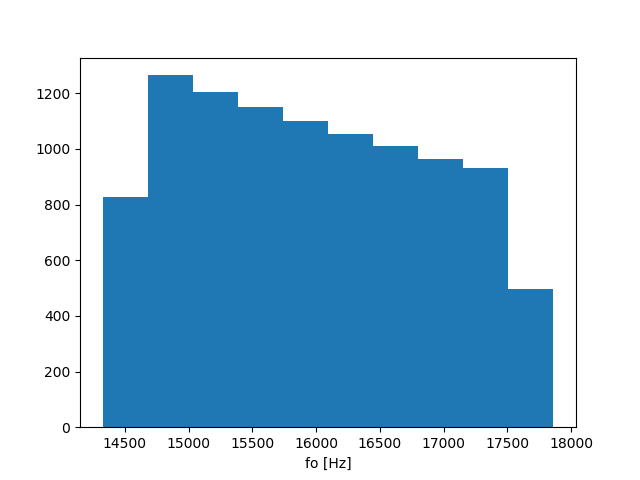
\includegraphics[scale=0.7]{../EJ1/Recursos/legendre_histogram_one.png}
    \caption{Histograma para la primera etapa de Legendre}
    \label{fig:legendre_histogram_one}
\end{figure}

\paragraph{$2^{\circ}$ etapa:} Se dise\~na una etapa de filtro pasabajo con los par\'ametros $\omega_o = 2 \pi \cdot 21.313kHz$ y $Q = 0.84$, obteniendo as\'i que se deb\'ia utilizar $R_1 = R_2 = 7.5k\Omega + 430 \Omega$ y $C_2 = 560pF$ y $C_1 = 1.5nF$.

\begin{figure}[H]
    \centering
    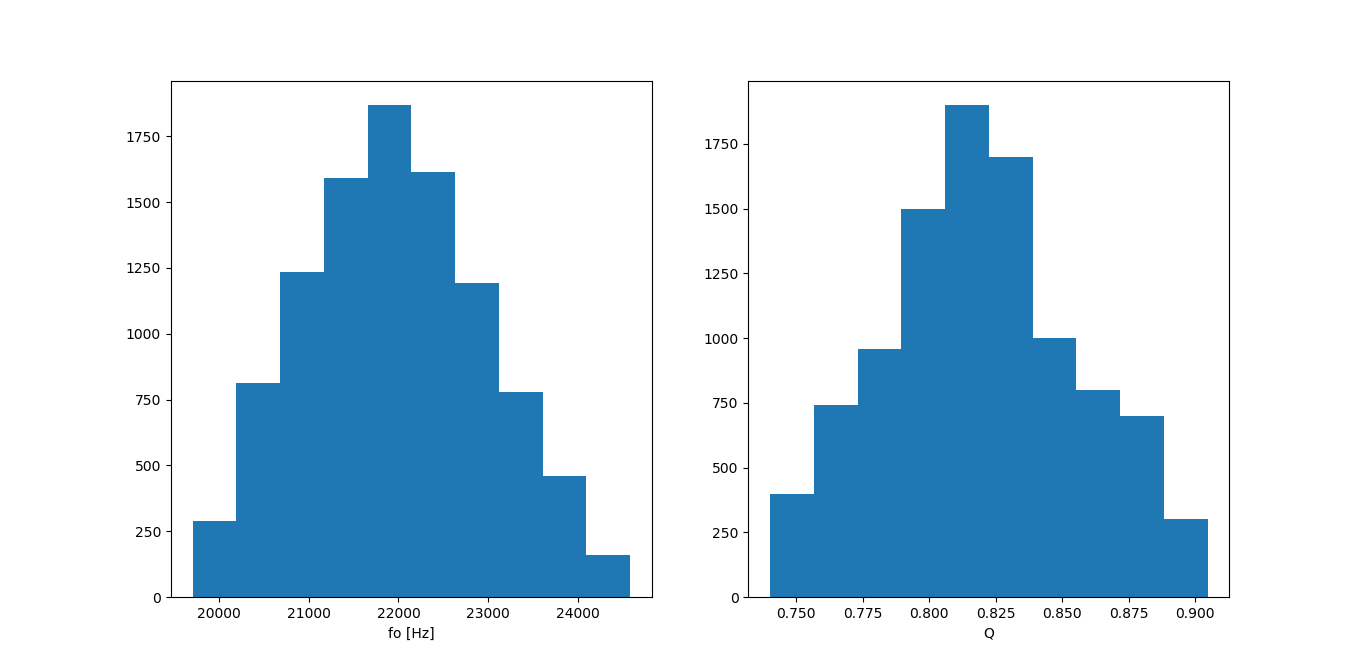
\includegraphics[scale=0.4]{../EJ1/Recursos/legendre_histogram_two.png}
    \caption{Histograma para la segunda etapa de Legendre}
    \label{fig:legendre_histogram_two}
\end{figure}

\paragraph{$3^{\circ}$ etapa:} Se dise\~na una etapa de filtro pasabajo con los par\'ametros $\omega_o = 2 \pi \cdot 28.371kHz$ y $Q = 2.88$, obteniendo as\'i que se deb\'ia utilizar $R_1 = R_2 = 9.1k\Omega + 620 \Omega$ y $C_2 = 100pF$ y $C_1 = 3.3nF$.

\begin{figure}[H]
    \centering
    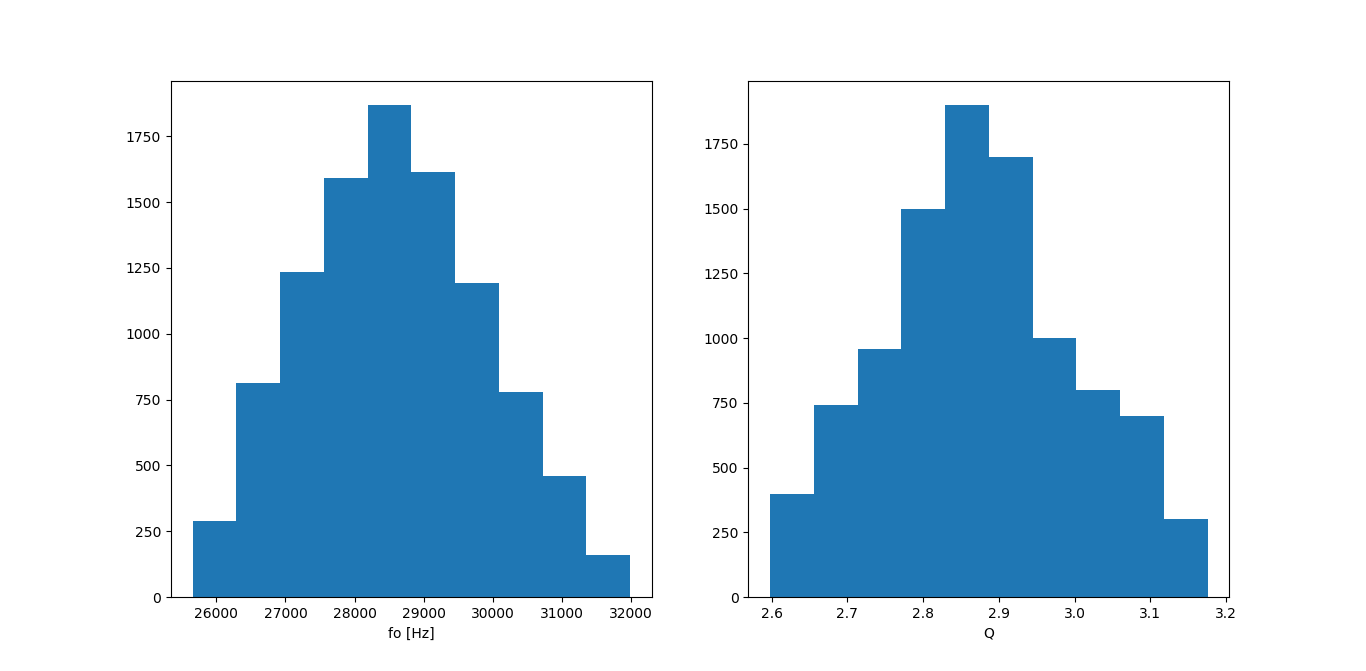
\includegraphics[scale=0.4]{../EJ1/Recursos/legendre_histogram_three.png}
    \caption{Histograma para la tercera etapa de Legendre}
    \label{fig:legendre_histogram_three}
\end{figure}

Para el dise\~no de las etapas se utiliza como amplificador operacional TL084 por su alto producto de ganancia y ancho de banda, as\'i como su alto slew rate, para garantizar una mayor regi\'on dentro de la cual se puede operar bajo condiciones ideales o asumiendo que lo son.

\subsubsection{Simulaci\'on y verificaci\'on}
Se realizan las simulaciones del filtro conectado en cascada utilizando las 3 etapas correspondientes, utilizando un an\'alisis de Monte Carlo se puede apreciar que ante las variaciones por tolerancias
de los componentes luego se cumple con la plantilla consignada en todo caso. Se puede observar que el orden del filtro es $n = 5$ en funci\'on del cambio de $450^{\circ}$ en la fase, $90^{\circ}$ por cada polo.

\begin{figure}[H]
    \centering
    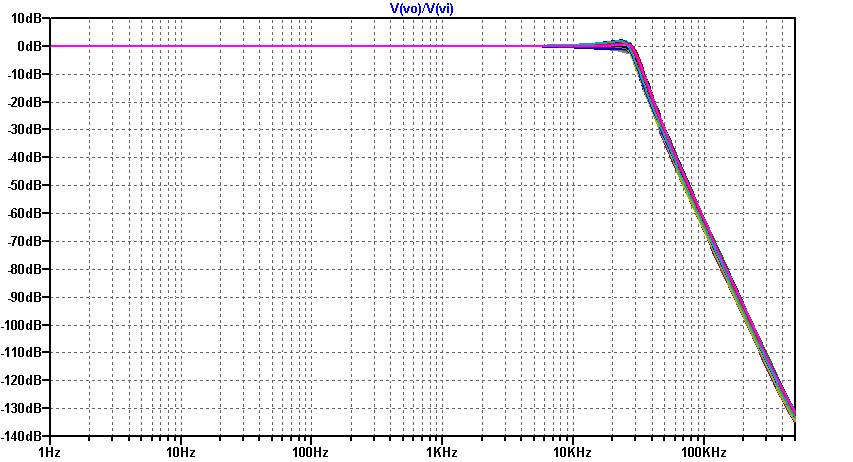
\includegraphics[scale=0.6]{../EJ1/Recursos/legendre_verificacion_magnitud.png}
    \caption{Diagrama de bode en m\'odulo simulado}
\end{figure}

\begin{figure}[H]
    \centering
    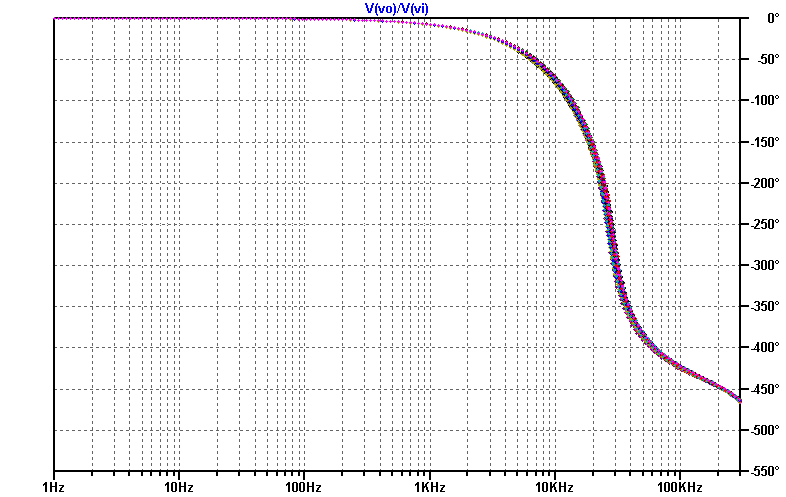
\includegraphics[scale=0.6]{../EJ1/Recursos/legendre_verificacion_fase.png}
    \caption{Diagrama de bode en fase simulado}
\end{figure}

\begin{figure}[H]
    \centering
    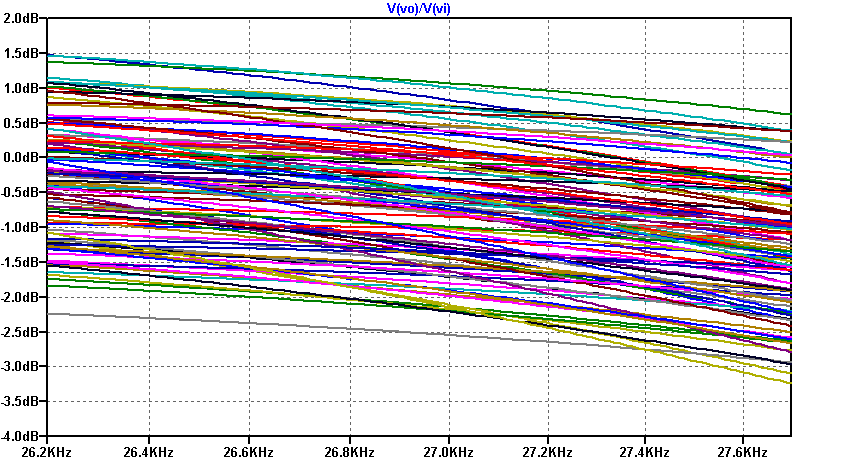
\includegraphics[scale=0.6]{../EJ1/Recursos/legendre_verificacion_fp.png}
    \caption{Verificaci\'on de la frecuencia de polo}
\end{figure}

\subsubsection{Resultados pr\'acticos}

\paragraph{Respuesta en frecuencia:} En las Figs. \ref{fig:legendre_bode_modulo} y \ref{fig:legendre_bode_fase} se pueden observar los resultados de la implementaci\'on
pr\'actica del filtro de Legendre con las celdas Sallen Key. Se realiza la contrastaci\'on de los resultados te\'oricos, pr\'acticos y simulados, acotando el rango de frecuencias
en donde se vuelvan apreciables las magnitudes medidas, ya que para mayores frecuencias la se\~nal de salida se encuentra atenuada por debajo del piso de ruido. Se puede observar que para
la frecuencia $f_p = 27kHz$ la ca\'ida medida es de $-1.73dB$.

\begin{figure}[H]
    \centering
    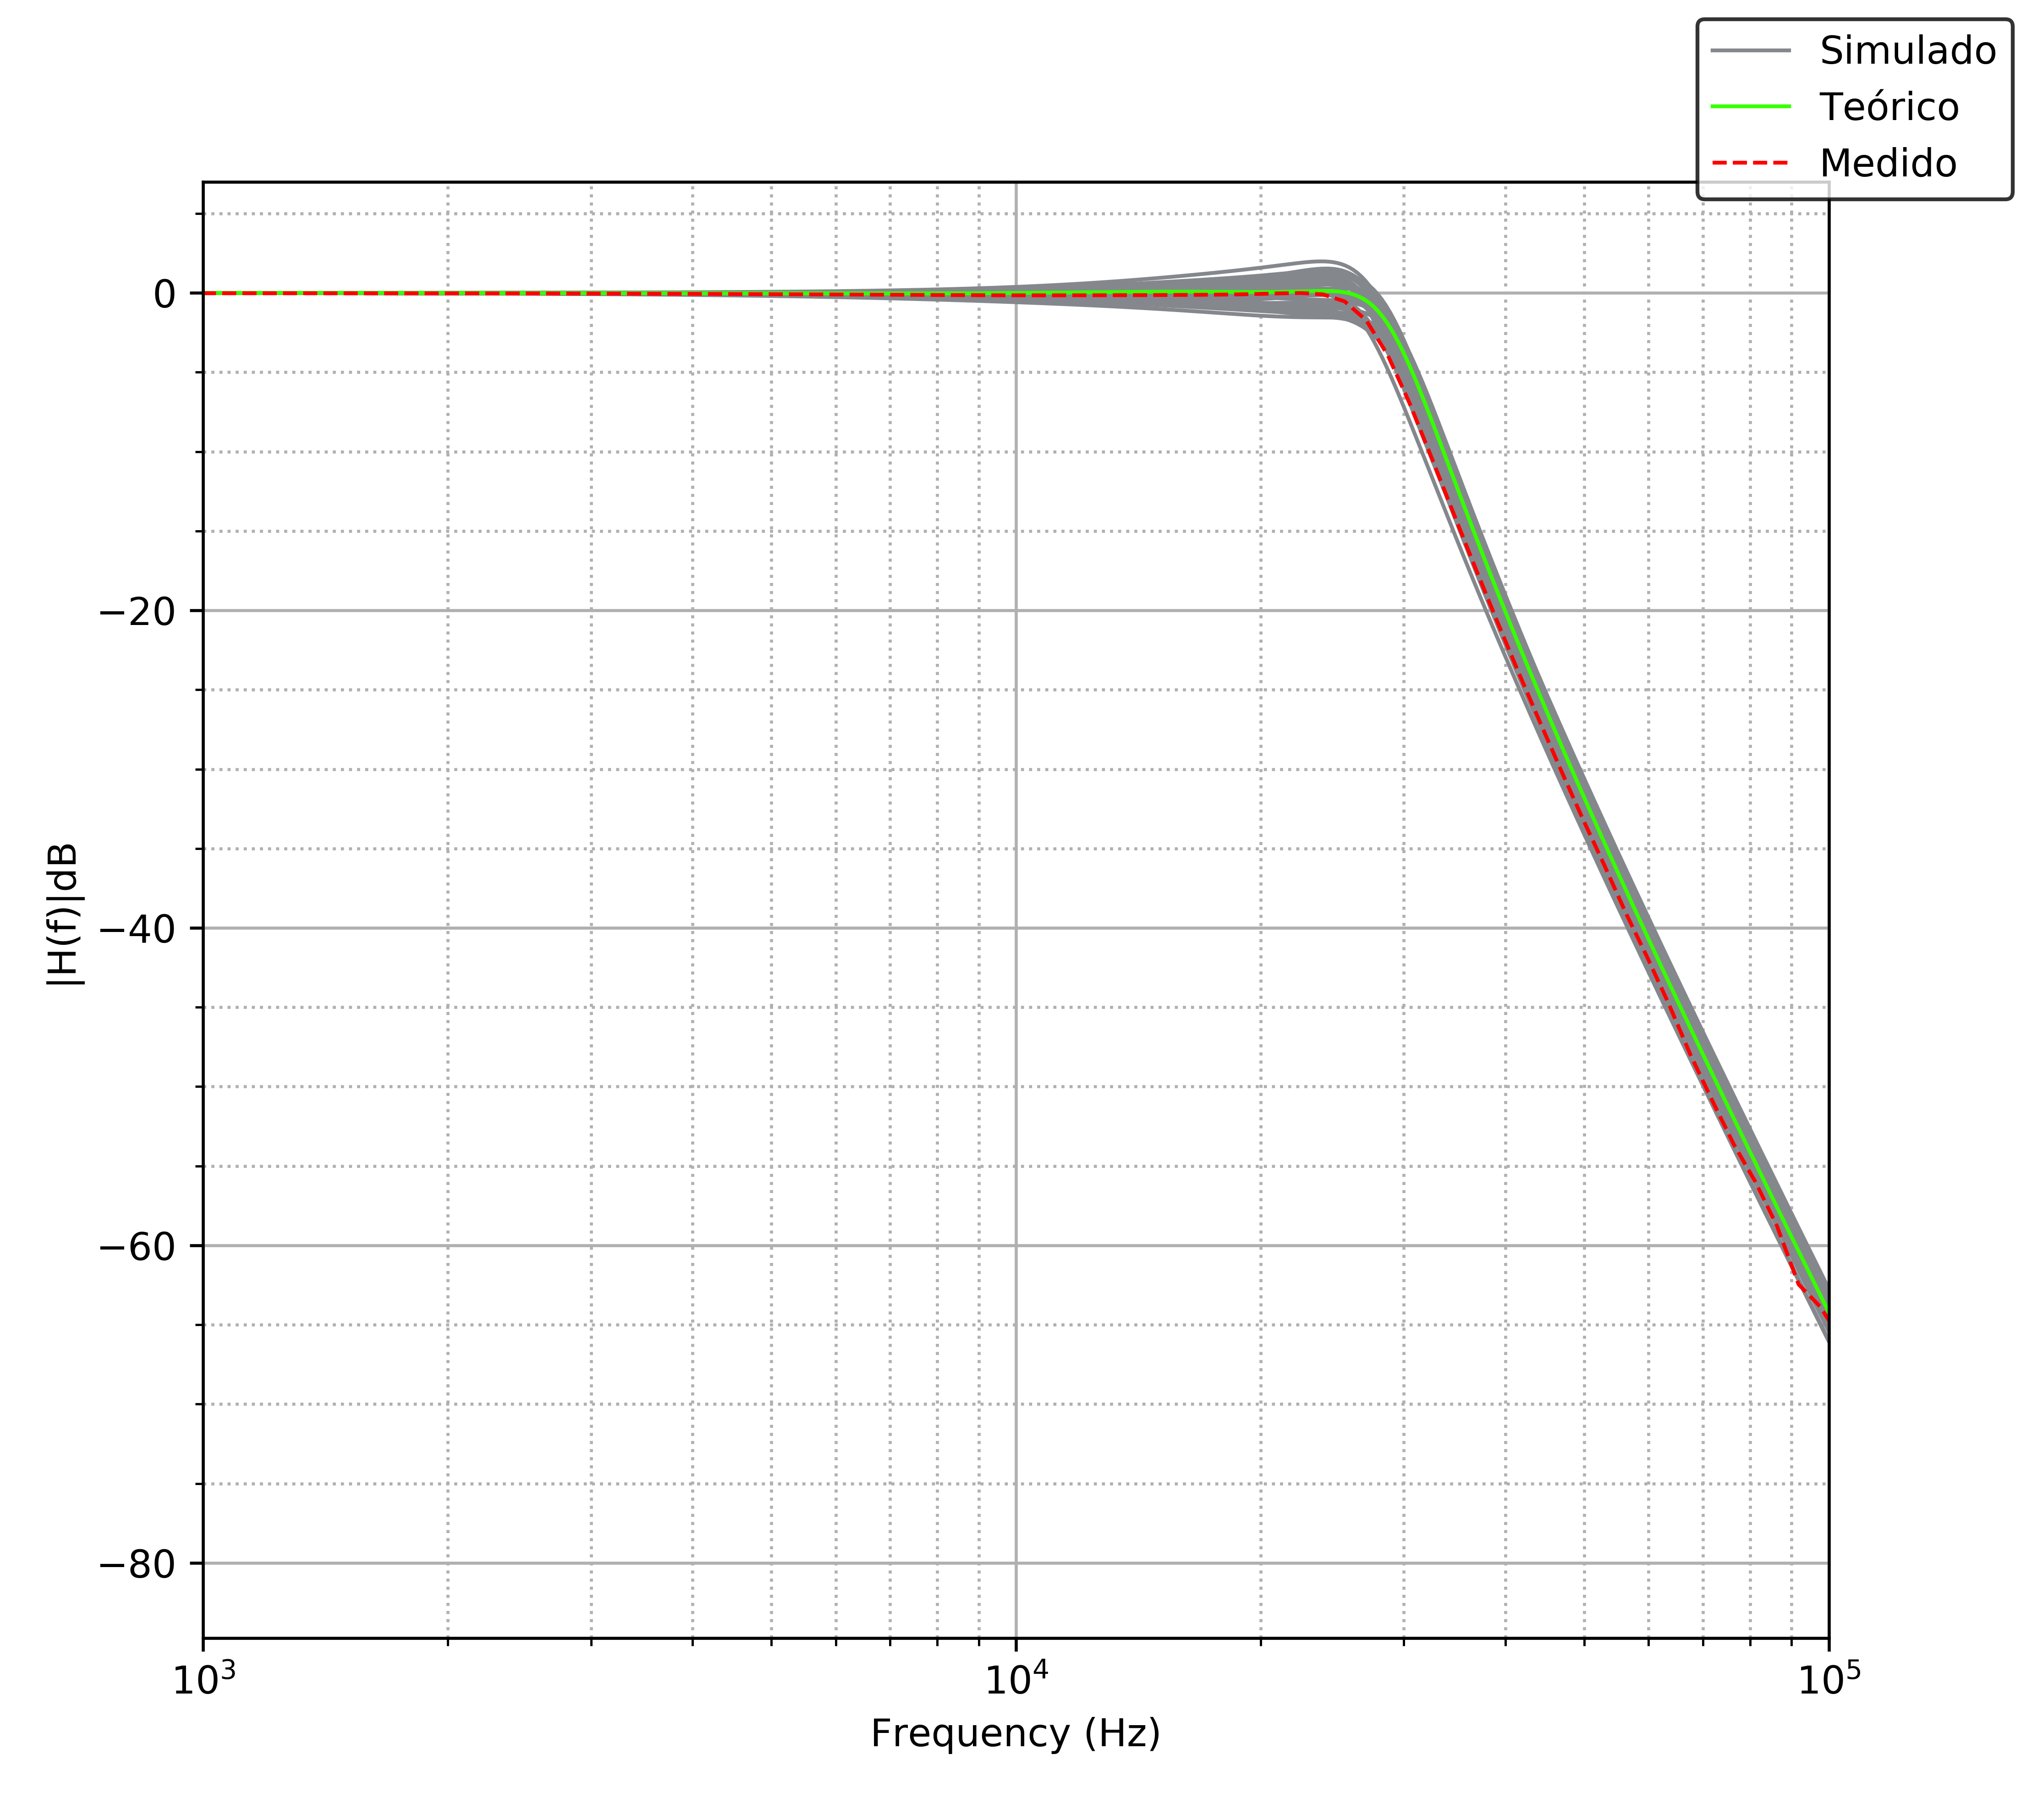
\includegraphics[scale=0.7]{../EJ1/Recursos/legendre_bode_modulo.png}
    \caption{Diagrama de bode en m\'odulo}
    \label{fig:legendre_bode_modulo}
\end{figure}

\begin{figure}[H]
    \centering
    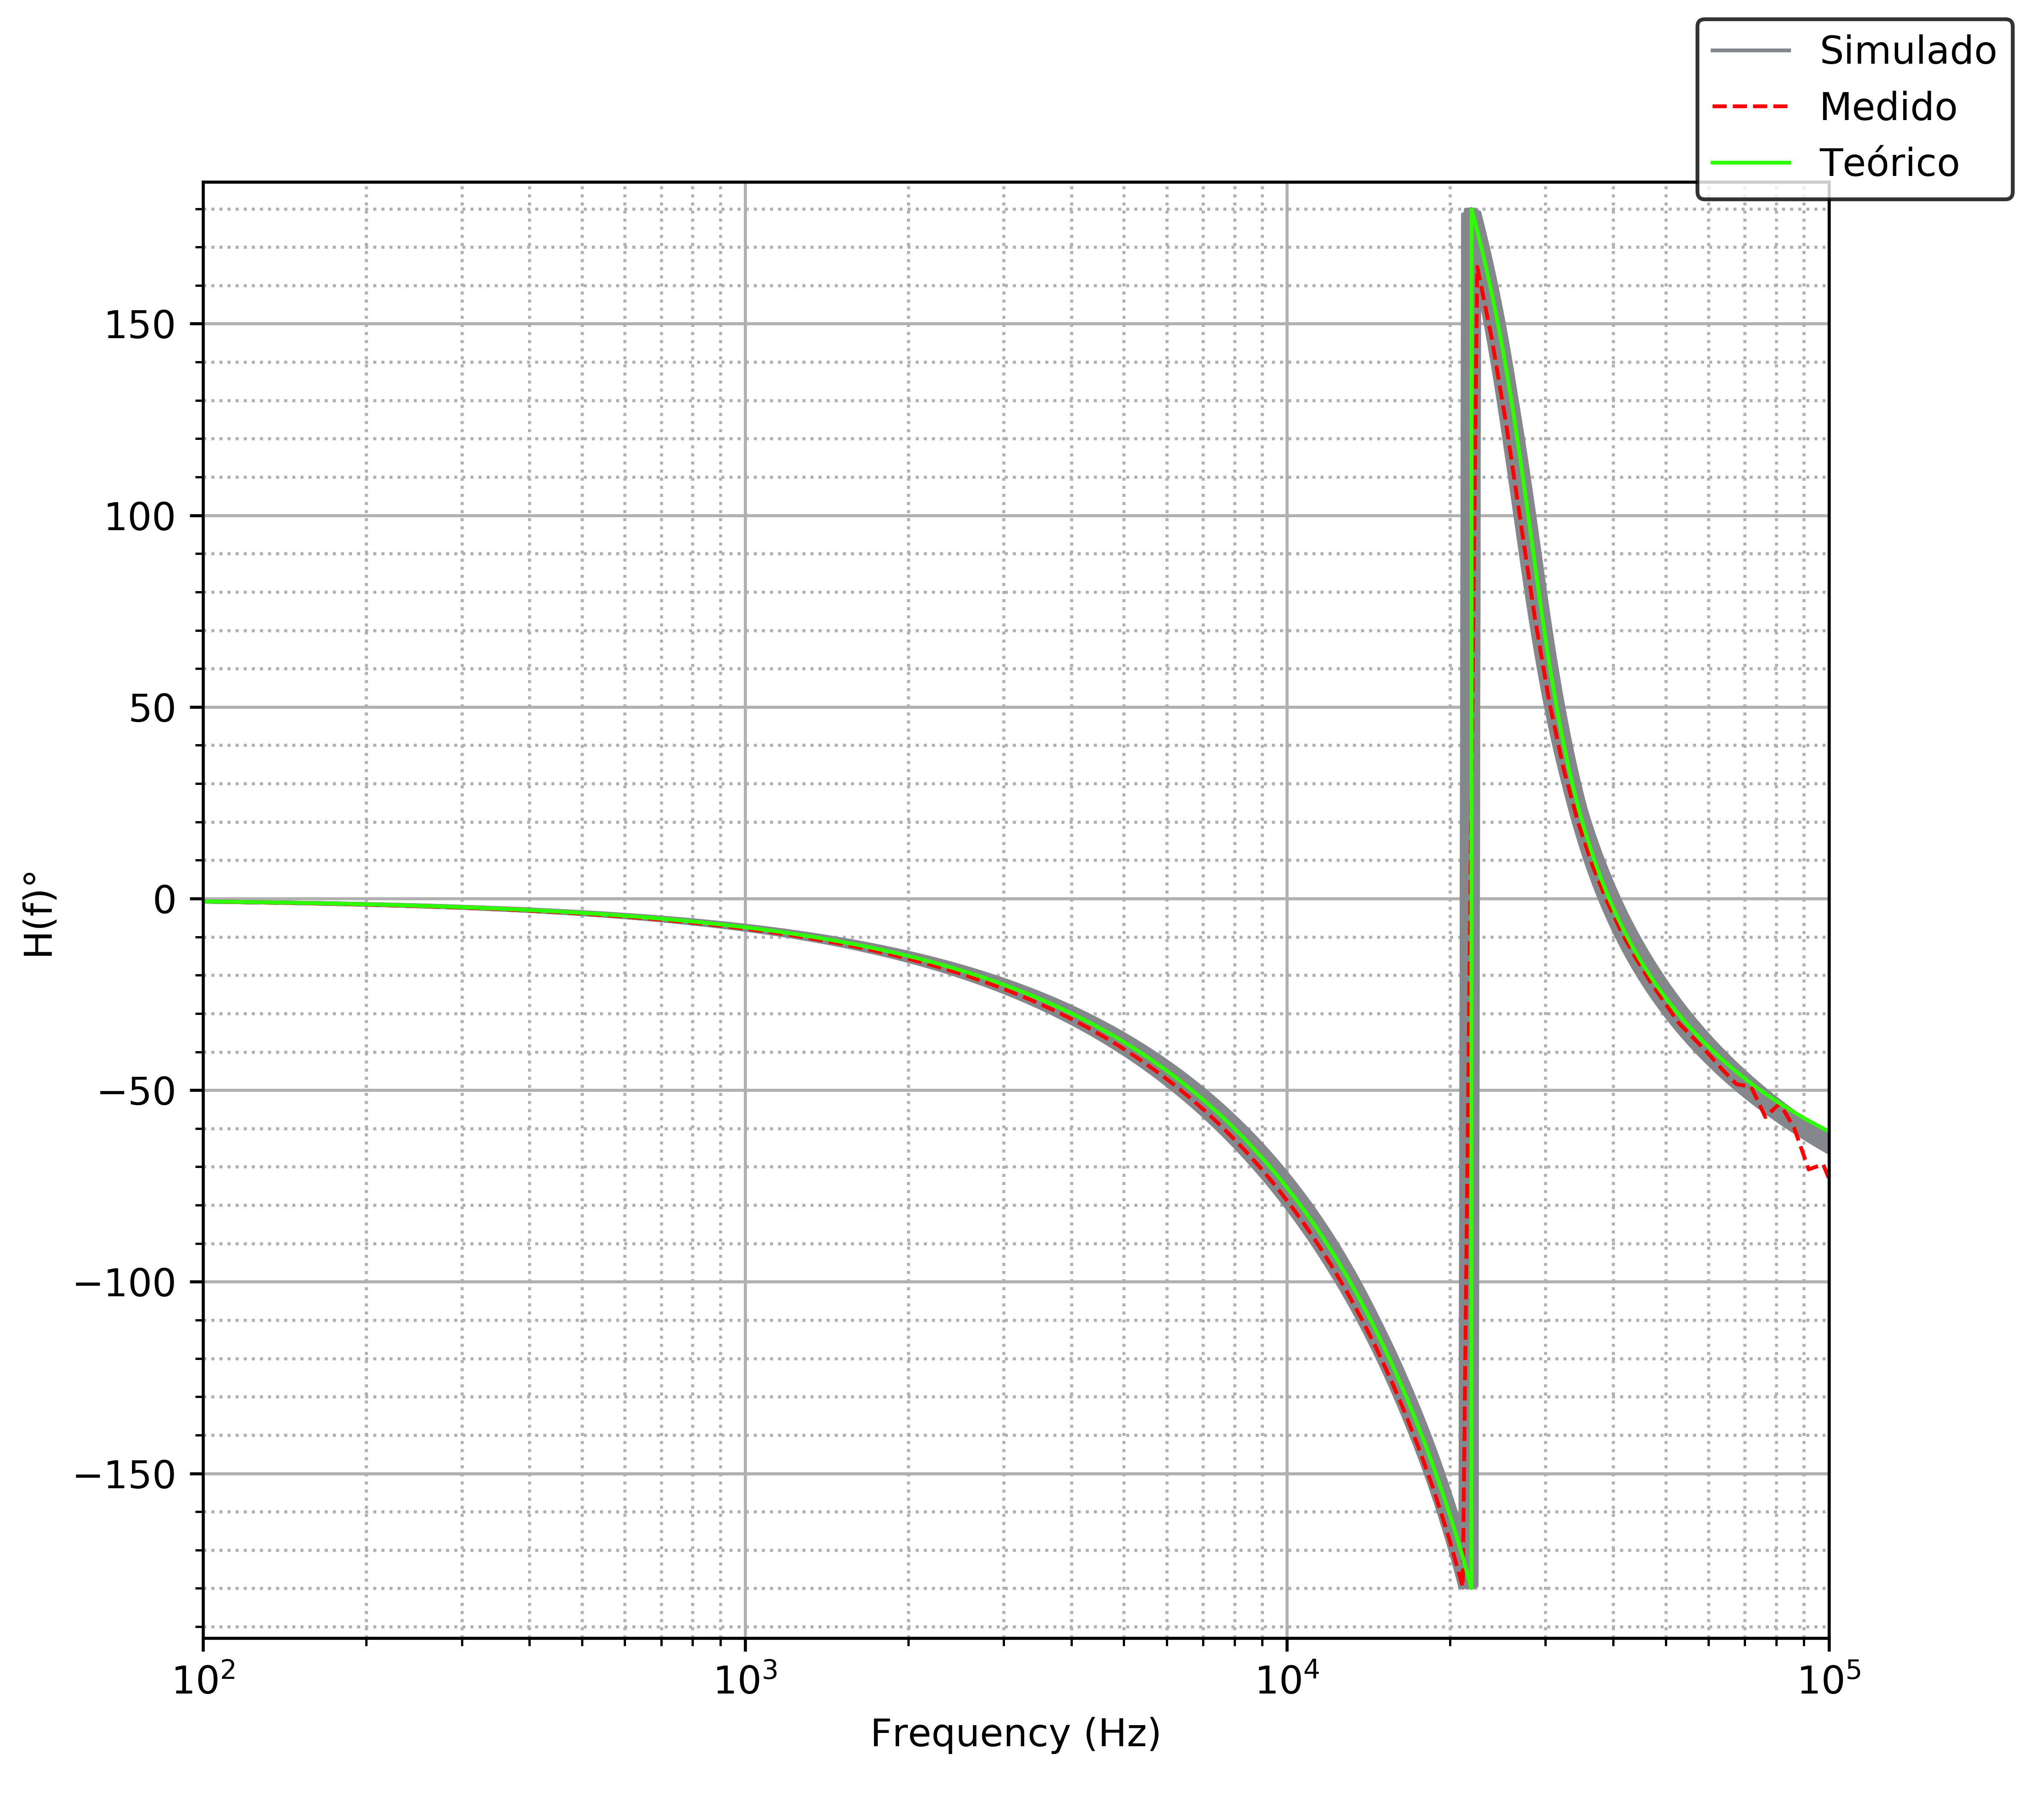
\includegraphics[scale=0.7]{../EJ1/Recursos/legendre_bode_fase.png}
    \caption{Diagrama de bode en fase}
    \label{fig:legendre_bode_fase}
\end{figure}

\paragraph{Impedancia de entrada:} En la Fig. \ref{fig:legendre_impedancia_entrada} se puede observar la impedancia de entrada medida para el circuito que implementa
el filtro de la aproximaci\'on de Legendre. Para menores frecuencias la impedancia era mayor, y para mayores frecuencias la impedancia se manten\'ia constante en un valor,
como se puede observar, $Z_{in} \approx 100k\Omega$.

\begin{figure}[H]
    \centering
    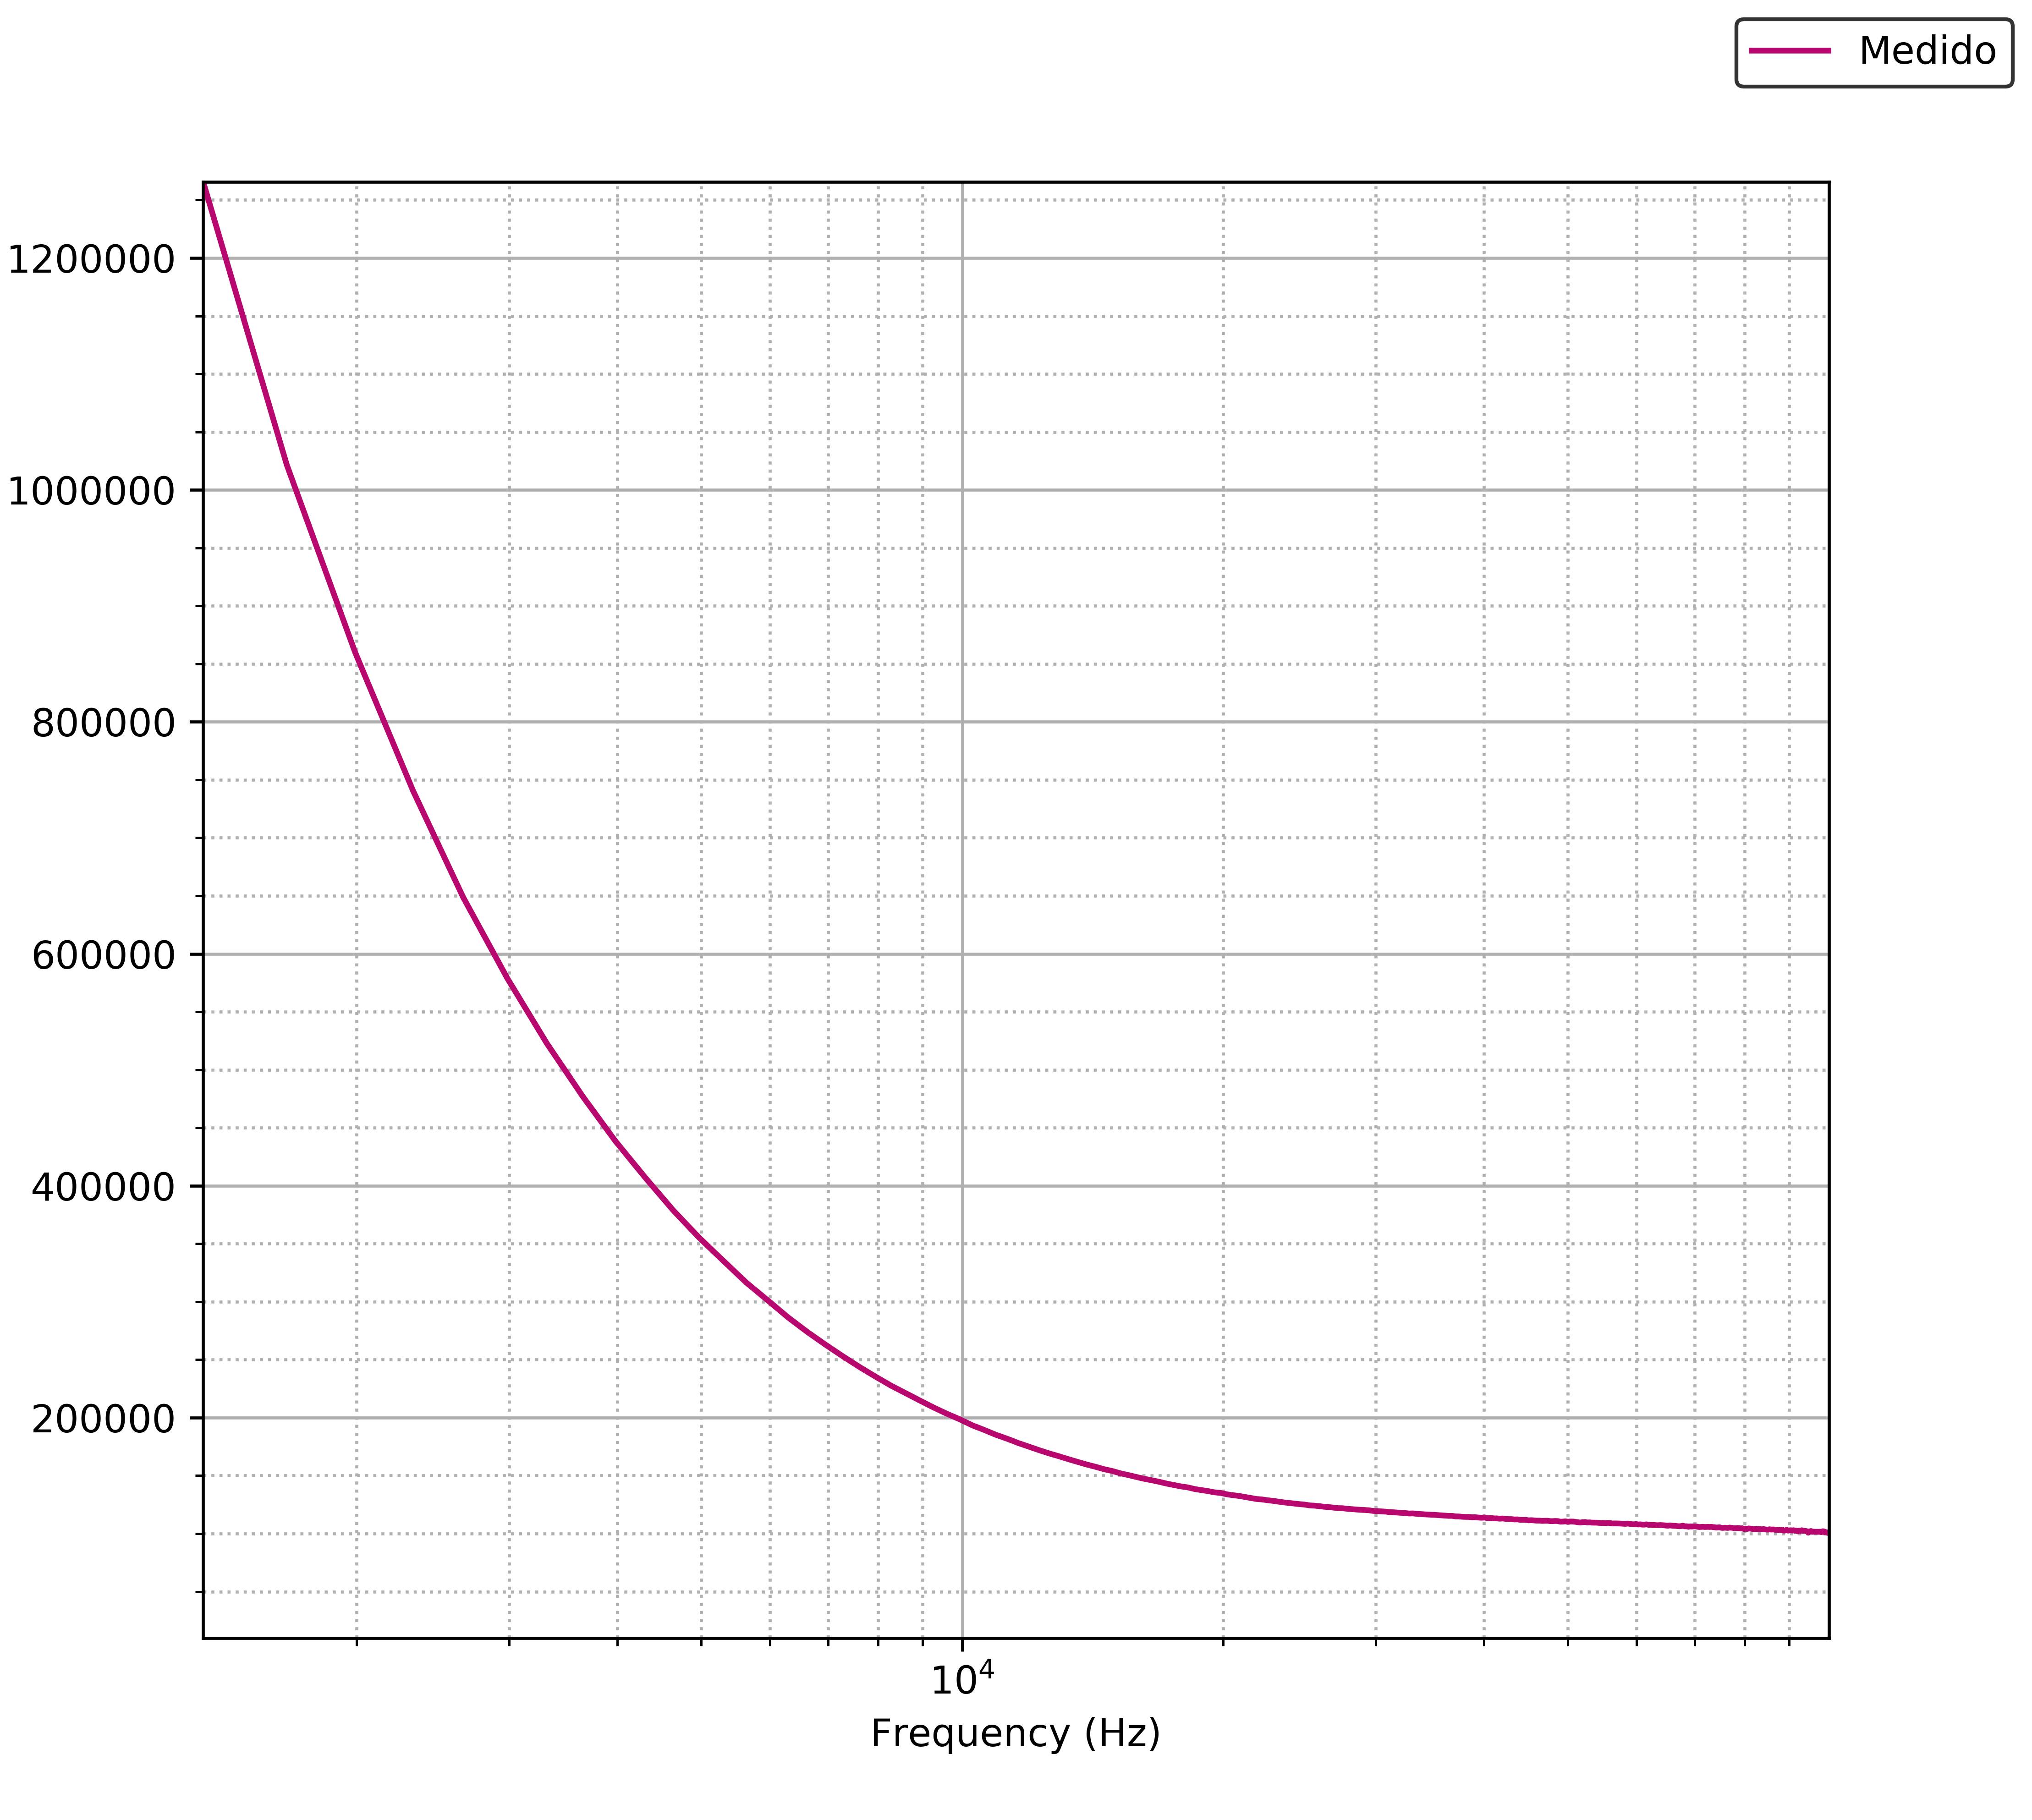
\includegraphics[scale=0.7]{../EJ1/Recursos/legendre_impedancia_entrada.png}
    \caption{Impedancia de entrada medida}
    \label{fig:legendre_impedancia_entrada}
\end{figure}

\subsection{Dise\~no de un filtro con Bessel}
La funci\'on de aproximaci\'on de Bessel se obtiene a partir de considerar una funci\'on racional como transferencia del sistema, a partir de la cual se realizan aproximaciones sobre la fase de su respuesta en frecuencia
buscando conseguir la modulaci\'on m\'as lineal posible, de esta forma por propiedades de la transformada de Fourier se puede garantizar que el retardo temporal que sufren las se\~nales que entran al sistema es constante
para un rango dado de frecuencias. Esta \'ultima es la ventaja principal de la aproximaci\'on de Bessel, no obstante, como consecuencia de tal an\'alisis adem\'as permite implementar un filtro pasabajos con tales caracter\'isticas.

Es importante mencionar que Bessel consigue la m\'axima planicie en el retardo de grupo, pero no existen expresiones cerradas para su c\'alculo, sino que dado un determinado orden de filtro se puede obtener la funci\'on transferencia
a partir de un c\'alculo recursivo, y de ah\'i es necesario verificar si cumple con las exigencias de las especificaciones del filtro a dise\~nar.

\begin{equation}
    H(s_N) = \frac{B_n(0)}{B_n(s_N)}
\end{equation}

En esta expresi\'on se emplean los polinomios de Bessel obtenidos de la ecuaci\'on recursiva de Bessel.

\subsubsection{Especificaciones y funci\'on aproximaci\'on}
Se desea dise\~nar un filtro pasabajos implementado con una funci\'on de Bessel para bajas se\~nales que cumpla con las especificaciones ilustradas
en la Tabla \ref{table:especificaciones_bessel}.

\begin{table}[H]
    \centering
    \begin{tabular}{c | c}
        \hline \\
        $f_p$ & $550Hz$ \\
        \\ \hline \\
        $f_a$ & $2600Hz$ \\
        \\ \hline \\
        $A_p$ & $3 dB$ \\
        \\ \hline \\
        $A_a$ & $40 dB$ \\
        \\ \hline \\
        $|Z_{IN}(f)|$ & $\geq 50k \Omega$ \\ 
        \\ \hline
        $|\gamma(f_p)|$ & $\leq 5 \% $ \\ 
        \\ \hline
    \end{tabular}
    \caption{Especificaciones de filtro con aproximaci\'on Bessel}
    \label{table:especificaciones_bessel}
\end{table}

A partir de estas especificaciones se debe iterar el orden de la funci\'on de Bessel hasta encontrar la $H(s_N)$ cuya pendiente en banda de transici\'on sea suficiente para cumplir con la plantilla
normalizada. Luego, es importante verificar que para dicho orden se cumple la m\'axima desviaci\'on admitida del retardo de grupo, que dicho sea de paso, no tiene restricci\'on alguna en su valor pero s\'i
en su variaci\'on porcentual respecto del valor constante esperado.


Finalmente, analizando la funci\'on de Bessel para cumplir con la plantilla de pasabajos y la m\'axima desviaci\'on del retardo de grupo, tomando cierto margen para evitar error por tolerancia de componentes,
se elige una funci\'on de orden $n = 6$.

\begin{table}[H]
    \centering
    \begin{tabular}{c | c}
        Polo & Ubicaci\'on \\
        \hline \\
        Complejo conjugado & $f_o = 1275.48Hz$ y $Q = 1.02$\\
        Complejo conjugado & $f_o = 1131.14Hz$ y $Q = 0.61$\\
        Complejo conjugado & $f_o = 1074.05Hz$ y $Q = 0.51$\\
        \\ \hline
    \end{tabular}
    \caption{Polos desnomarlizados de la $H(s)$}
\end{table}

\subsubsection{Dise\~no de etapas}
Para el dise\~no de este filtro se divide la funci\'on transferencia en tres diferentes etapas de segundo orden, donde se asume que se cumple la condici\'on necesaria para la conexi\'on en cascada,
esto es, que no se carguen las etapas entre s\'i en funci\'on de que sus impedancias de entrada son lo suficientemente grandes para lograr este objetivo. Por otro lado, se impone como restricci\'on que la impedancia de entrada
del circuito total sea $Z_{IN}(f) \geq 50k \Omega$, para esto \'ultimo se puede considerar la aproximaci\'on obtenida en el an\'alisis ideal, o suponiendo como peor caso considerar que para frecuencias muy grandes la impedancia m\'as chica
depende directamente de las resistencia en la entrada, con lo cual eso determinar\'a el l\'imite inferior en la selecci\'on de sus valores. Finalmente, este filtro es para se\~nales bajas con lo cual se ordenan los filtros de forma tal que se encuentren ordenados
de menor a mayor atenuaci\'on para evitar bajar la se\~nal a los niveles del ruido.

\paragraph{$1^{\circ} etapa:$} Se dise\~na un filtro de segundo orden pasabajos con requisitos $f_0 = 1074.05Hz$ y $Q = 0.51$, empleando la celda Sallen-Key se llega a los valores $R_1 = R_2 = 120k \Omega + 1k\Omega$, $C_1 = 1.2nF$ y $C_2 = 1.2nF$

\begin{figure}[H]
    \centering
    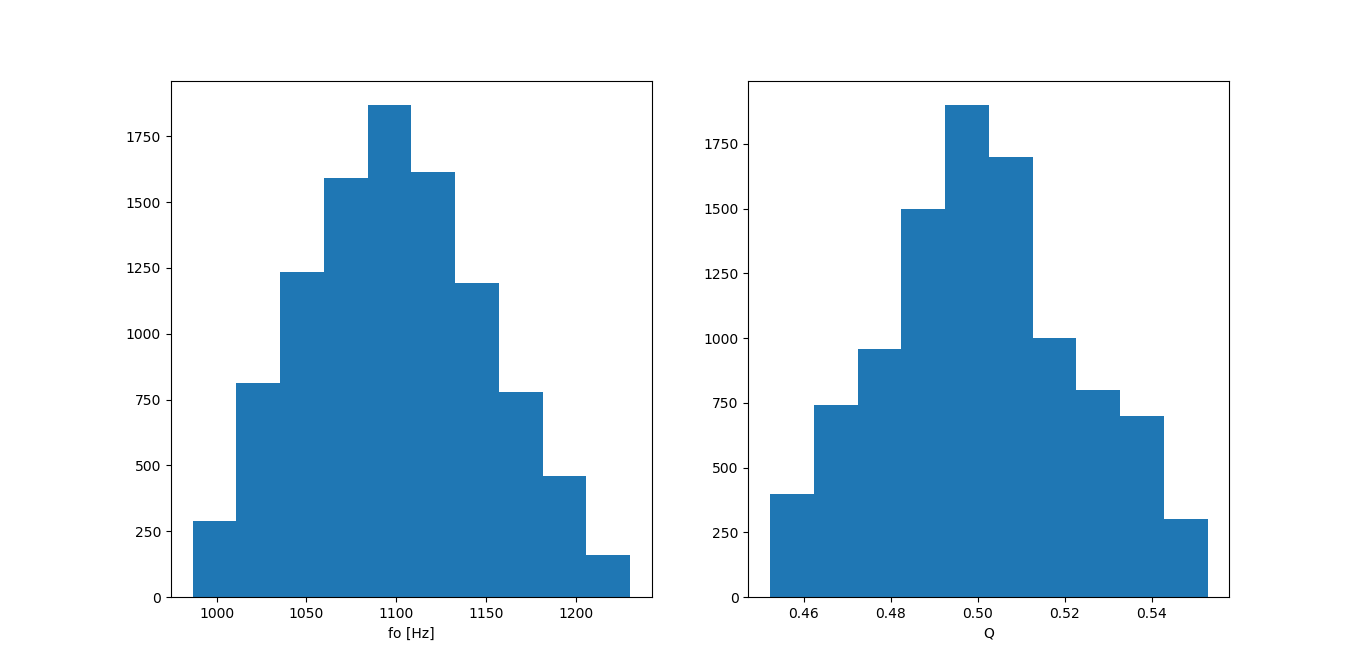
\includegraphics[scale=0.4]{../EJ1/Recursos/bessel_histogram_one.png}
    \caption{Histograma para la primer etapa de Bessel}
    \label{fig:bessel_histogram_one}
\end{figure}

\paragraph{$2^{\circ} etapa:$} Se dise\~na un filtro de segundo orden pasabajos con requisitos $f_0 = 1131.14Hz$ y $Q = 0.61$, empleando la celda Sallen-Key se llega a los valores $R_1 = R_2 = 75k \Omega + 1k8\Omega$, $C_1 = 2.2nF$ y $C_2 = 1.5nF$

\begin{figure}[H]
    \centering
    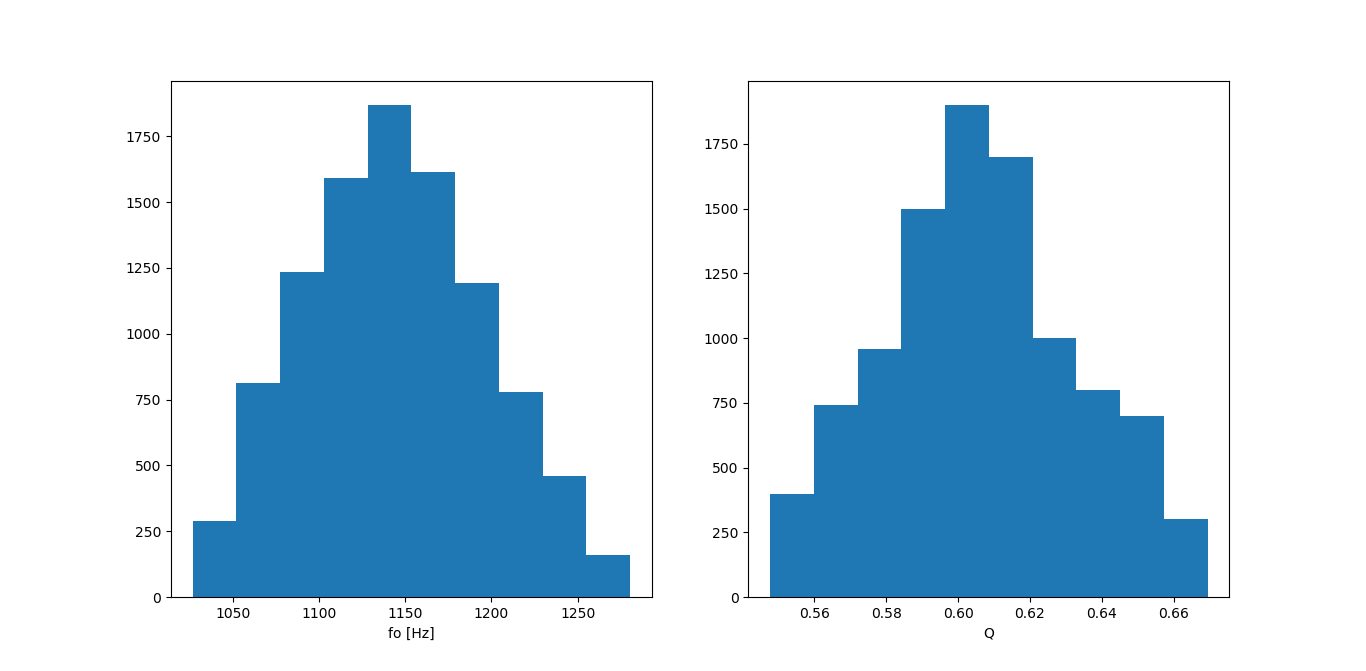
\includegraphics[scale=0.4]{../EJ1/Recursos/bessel_histogram_two.png}
    \caption{Histograma para la segunda etapa de Bessel}
    \label{fig:bessel_histogram_two}
\end{figure}

\paragraph{$3^{\circ} etapa:$} Se dise\~na un filtro de segundo orden pasabajos con requisitos $f_0 = 1275.48Hz$ y $Q = 1.02$, empleando la celda Sallen-Key se llega a los valores $R_1 = R_2 = 22k \Omega + 680\Omega$, $C_1 = 12nF$ y $C_2 = 2.7nF$.

\begin{figure}[H]
    \centering
    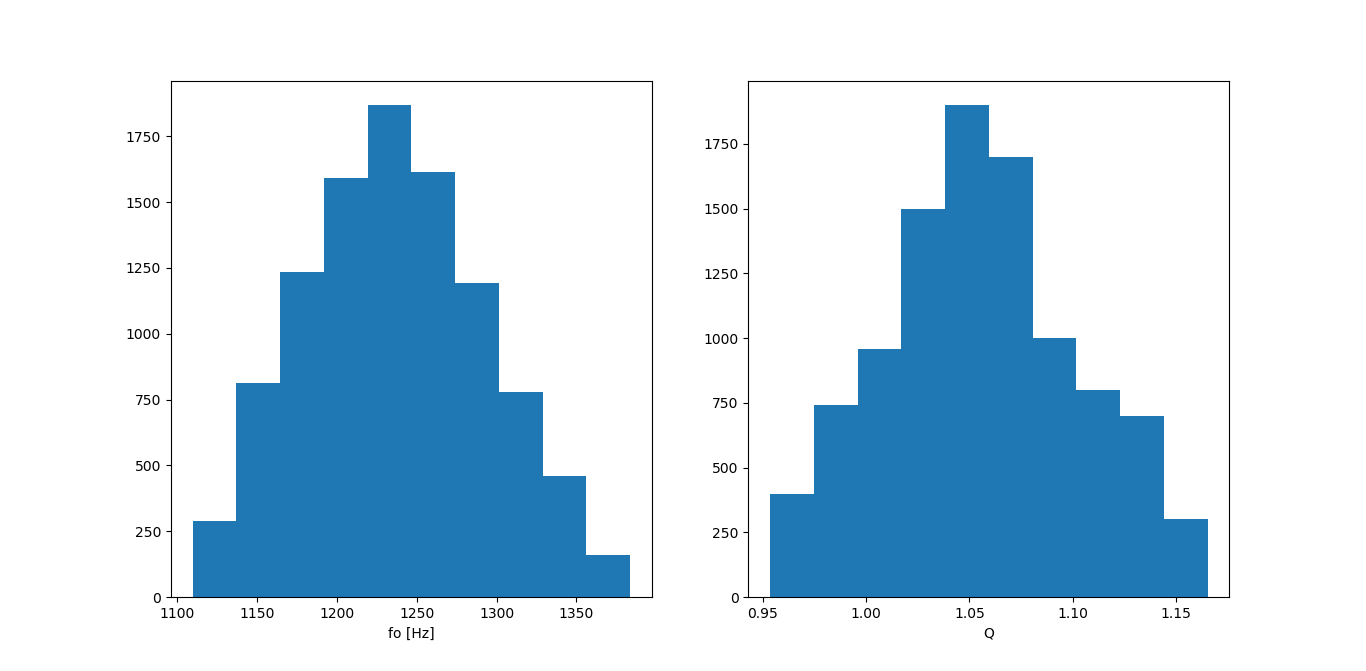
\includegraphics[scale=0.4]{../EJ1/Recursos/bessel_histogram_three.png}
    \caption{Histograma para la tercera etapa de Bessel}
    \label{fig:bessel_histogram_three}
\end{figure}

Al igual que para el filtro de Legendre, para maximizar el ancho de banda del circuito se emplea el operacional disponible con mayor producto de ganancia y ancho de banda, que adem\'as disponga de 4 operacionales y una gran impedancia de entrada, este es el TL084.

\subsubsection{Simulaci\'on y verificaci\'on}
Se realizan las simulaciones utilizando un an\'alisis de Monte Carlo para contemplar las variaciones respecto de los valores nominales de los componentes por sus tolerancias,
se puede observar en la fase que el sistema es de sexto orden dado el cambio de fase correspondiente.

\begin{figure}[H]
    \centering
    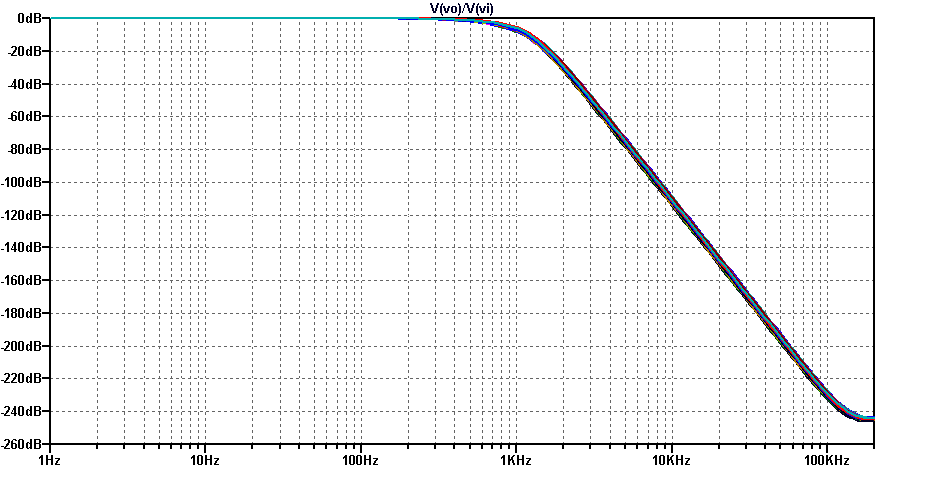
\includegraphics[scale=0.6]{../EJ1/Recursos/bessel_verificacion_magnitud.png}
    \caption{Verificaci\'on de la frecuencia de rechazo}
\end{figure}

\begin{figure}[H]
    \centering
    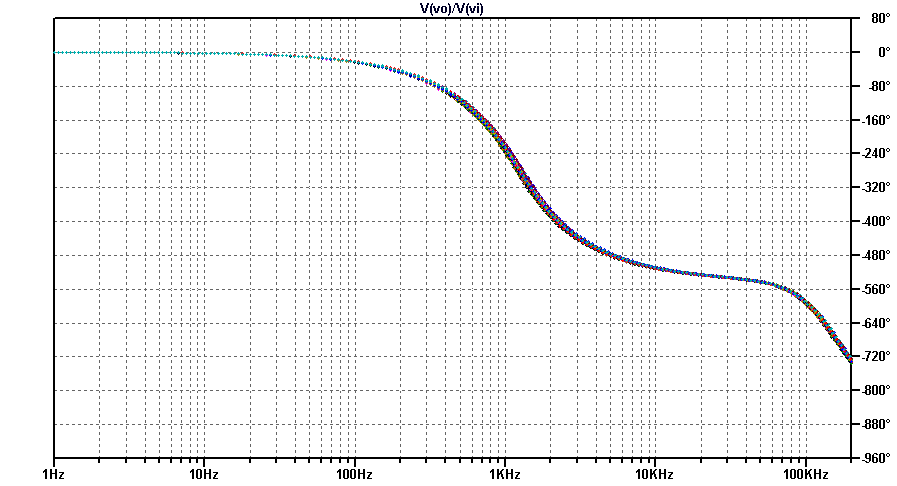
\includegraphics[scale=0.6]{../EJ1/Recursos/bessel_verificacion_fase.png}
    \caption{Verificaci\'on de la frecuencia de rechazo}
\end{figure}

\begin{figure}[H]
    \centering
    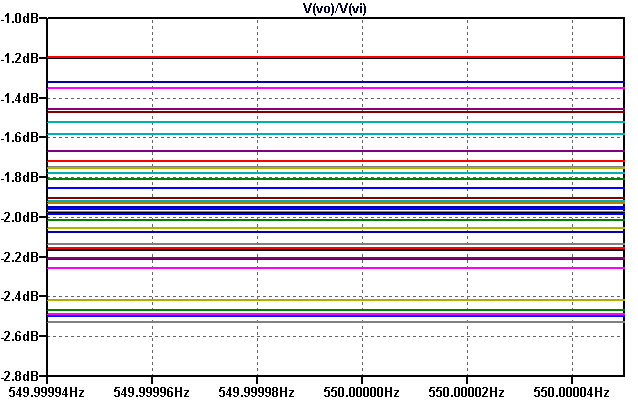
\includegraphics[scale=0.6]{../EJ1/Recursos/bessel_verificacion_fp.png}
    \caption{Verificaci\'on de la frecuencia de paso}
\end{figure}

\begin{figure}[H]
    \centering
    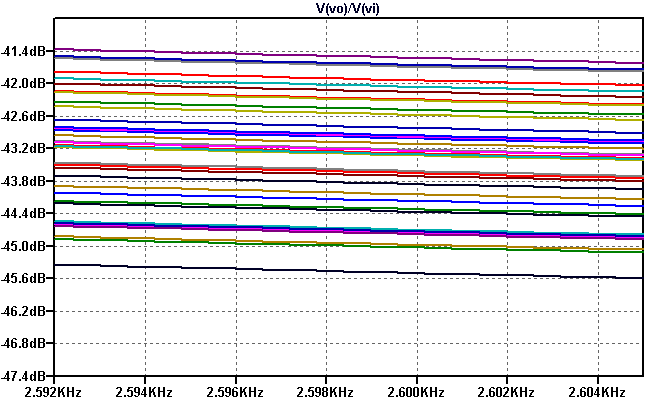
\includegraphics[scale=0.6]{../EJ1/Recursos/bessel_verificacion_fa.png}
    \caption{Verificaci\'on de la frecuencia de rechazo}
\end{figure}

\subsubsection{Resultados pr\'acticos}

\paragraph{Respuesta en frecuencia:} En las Figs. \ref{fig:bessel_bode_modulo} y \ref{fig:bessel_bode_fase} se pueden observar los resultados
contrastados entre la teor\'ia, la pr\'actica y lo simulado, donde el rango de frecuencia se restringe dado que para mayores frecuencias la atenuaci\'on
provocaba que la salida se encontrase por debajo del piso del ruido. Se puede observar que para $f_p = 550Hz$ la ca\'ida medida es de $-2.1dB$ y para $f_a = 2600Hz$ la ca\'ida
medida es de $-44.4dB$.

\begin{figure}[H]
    \centering
    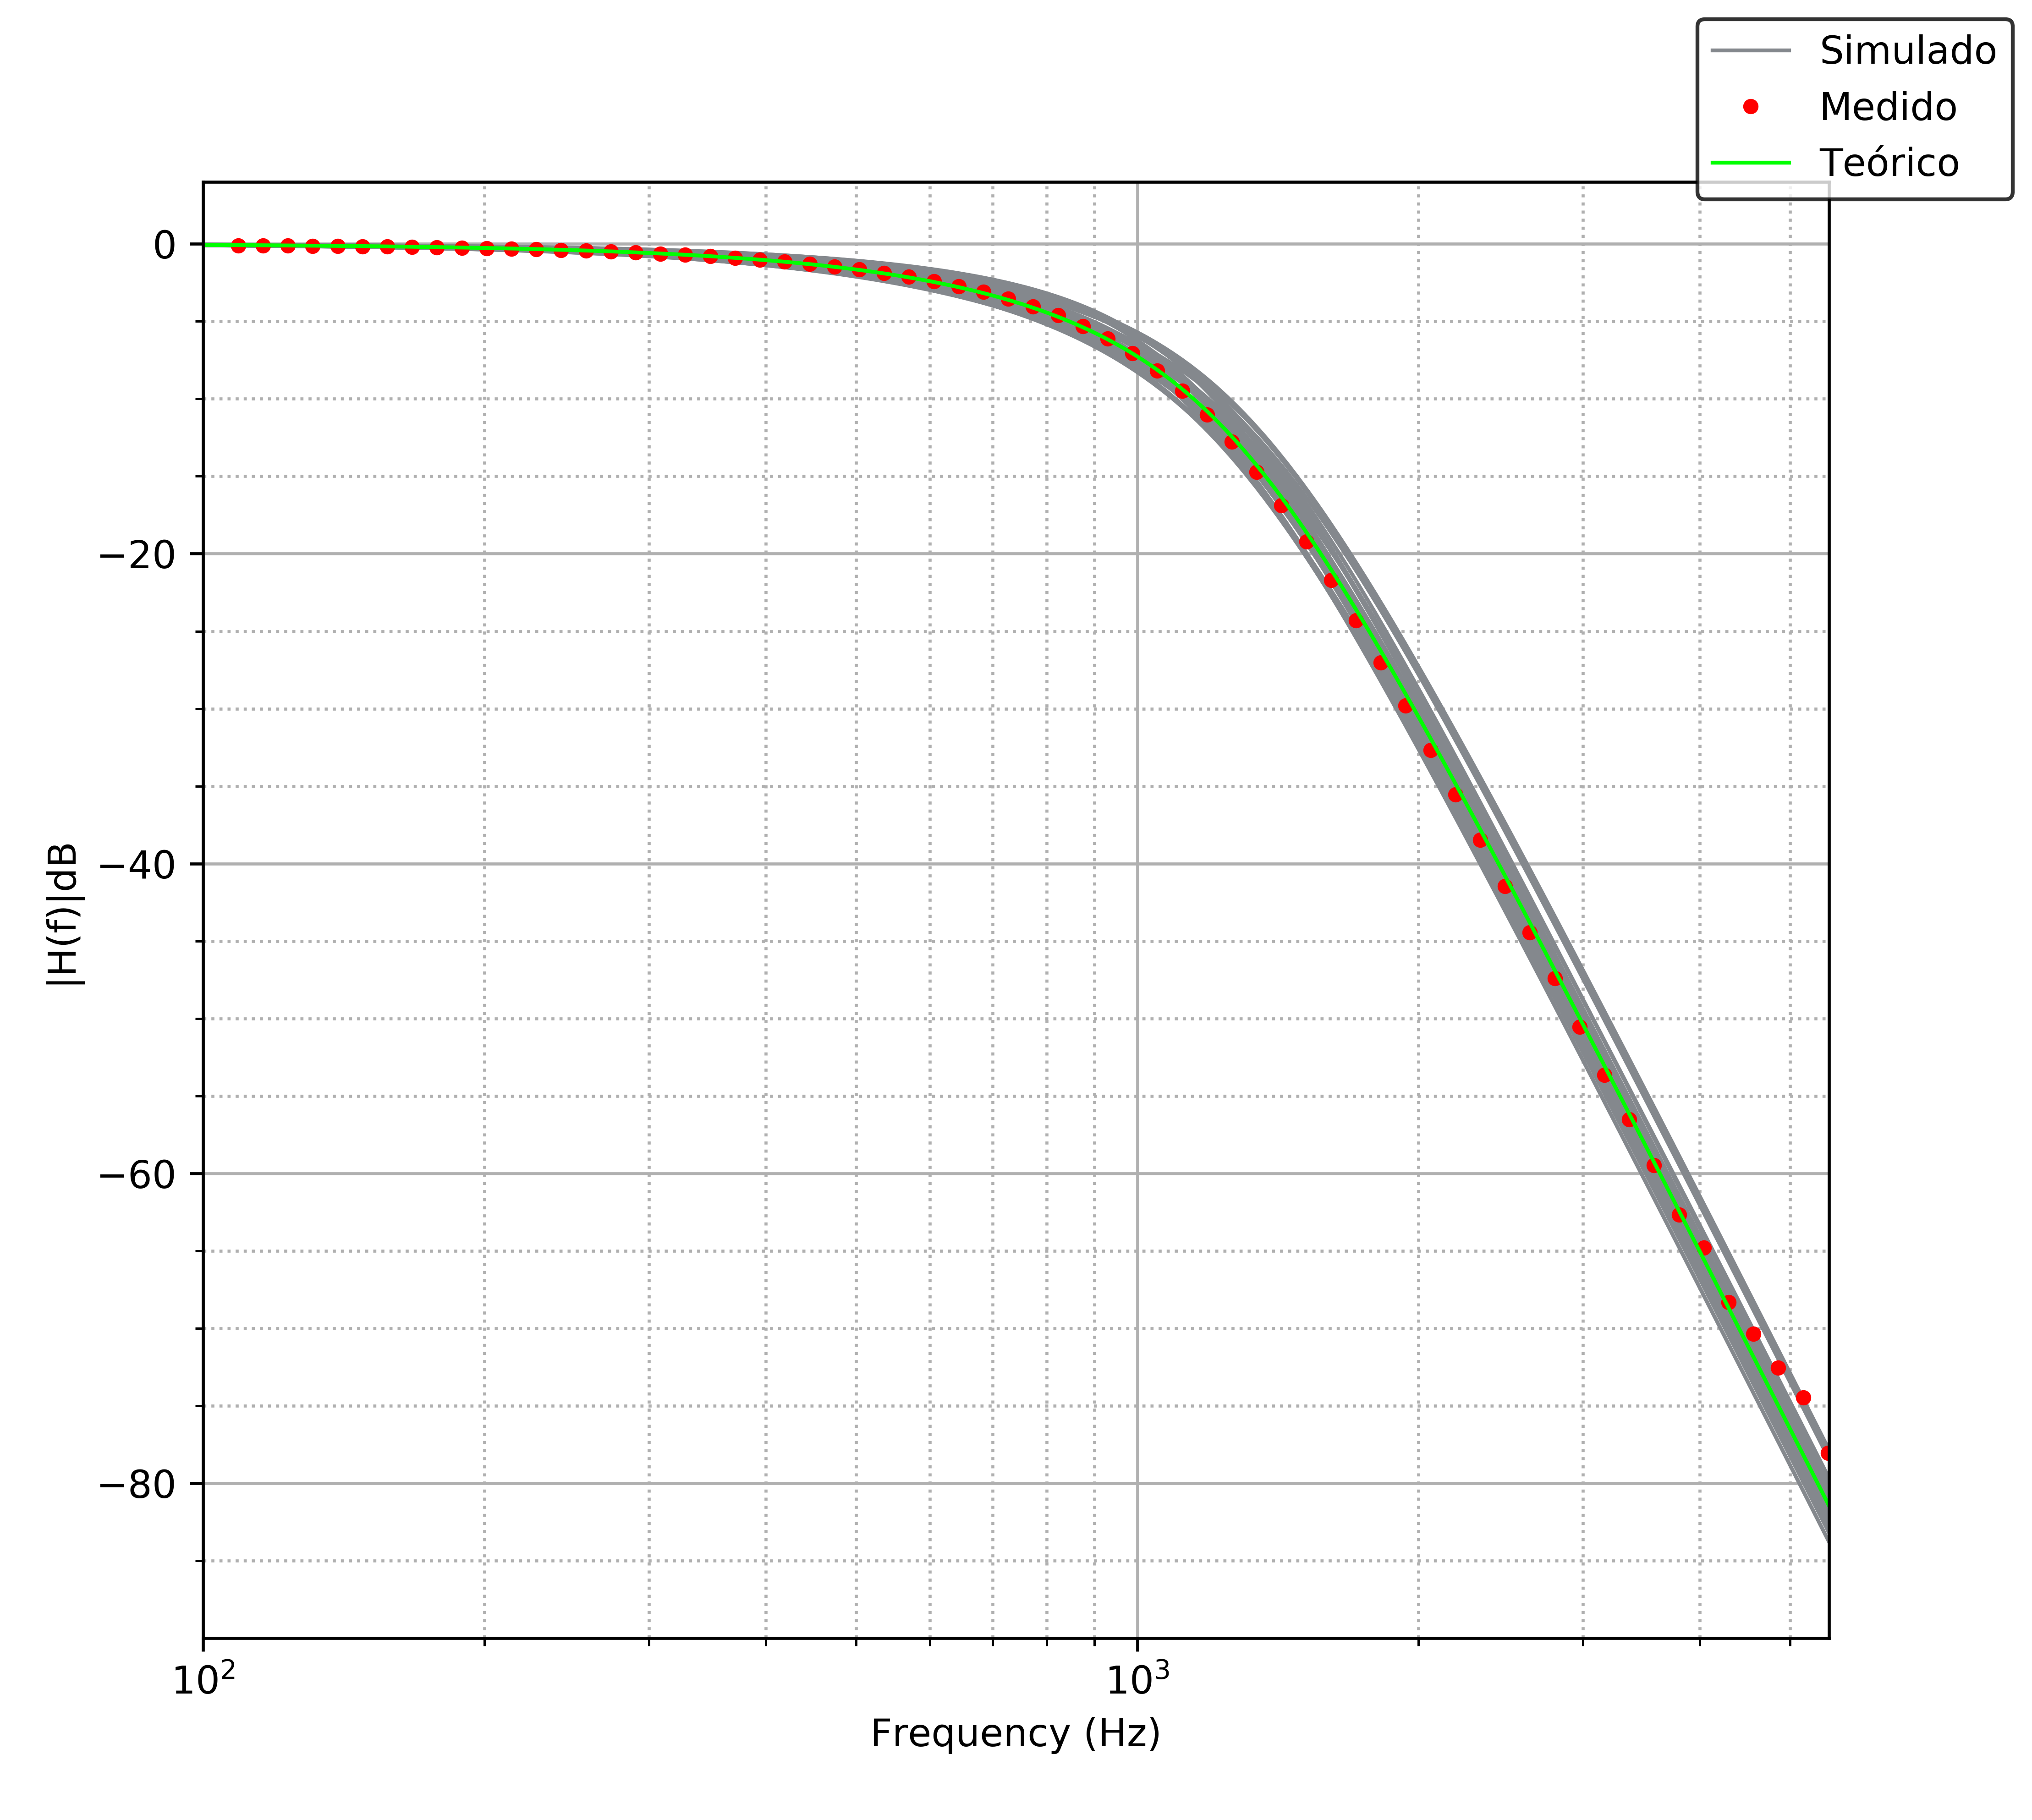
\includegraphics[scale=0.7]{../EJ1/Recursos/bessel_bode_modula.png}
    \caption{Diagrama de bode en m\'odulo}
    \label{fig:bessel_bode_modulo}
\end{figure}

\begin{figure}[H]
    \centering
    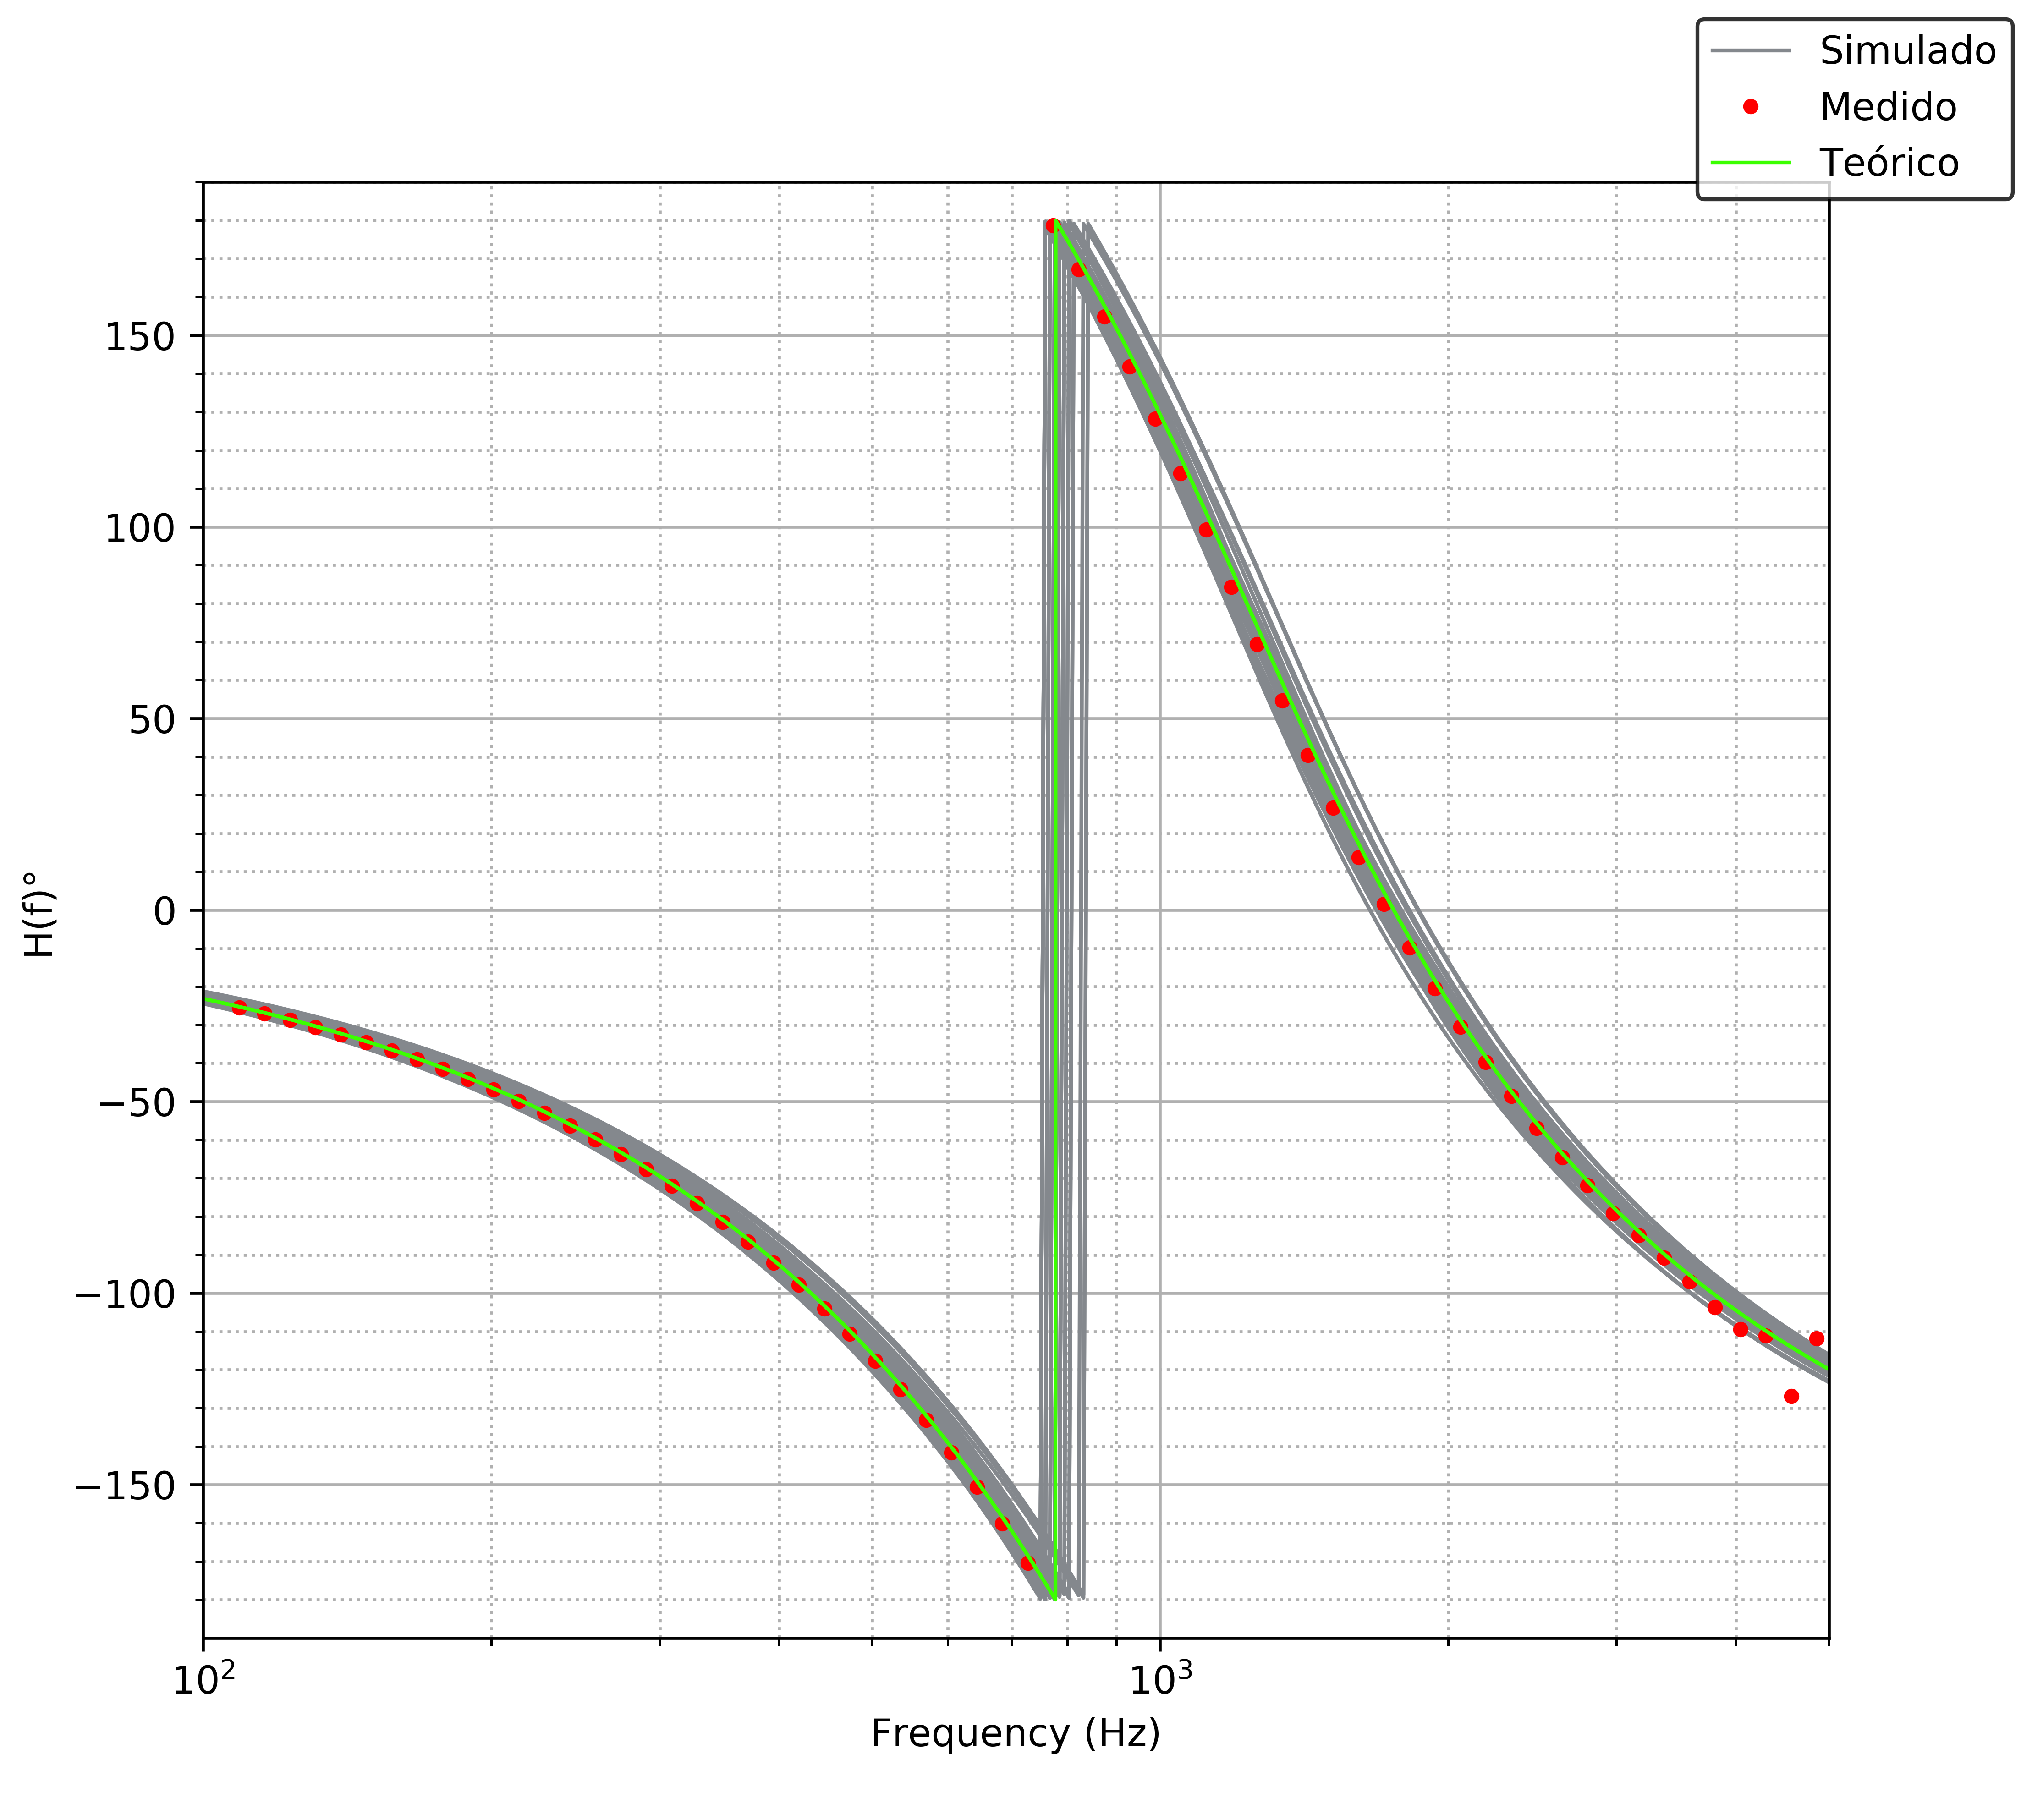
\includegraphics[scale=0.7]{../EJ1/Recursos/bessel_bode_fase.png}
    \caption{Diagrama de bode en fase}
    \label{fig:bessel_bode_fase}
\end{figure}

\paragraph{Impedancia de entrada:} En la Fig. \ref{bessel_impedancia_entrada} se puede observar la impedancia de entrada del circuito, donde para menores frecuencias
el valor era mayor, mientras que para mayores frecuencias se manten\'ia casi constante, siempre por encima del valor m\'inimo que puede observarse como $Z_{in} = 127k\Omega$.

\begin{figure}[H]
    \centering
    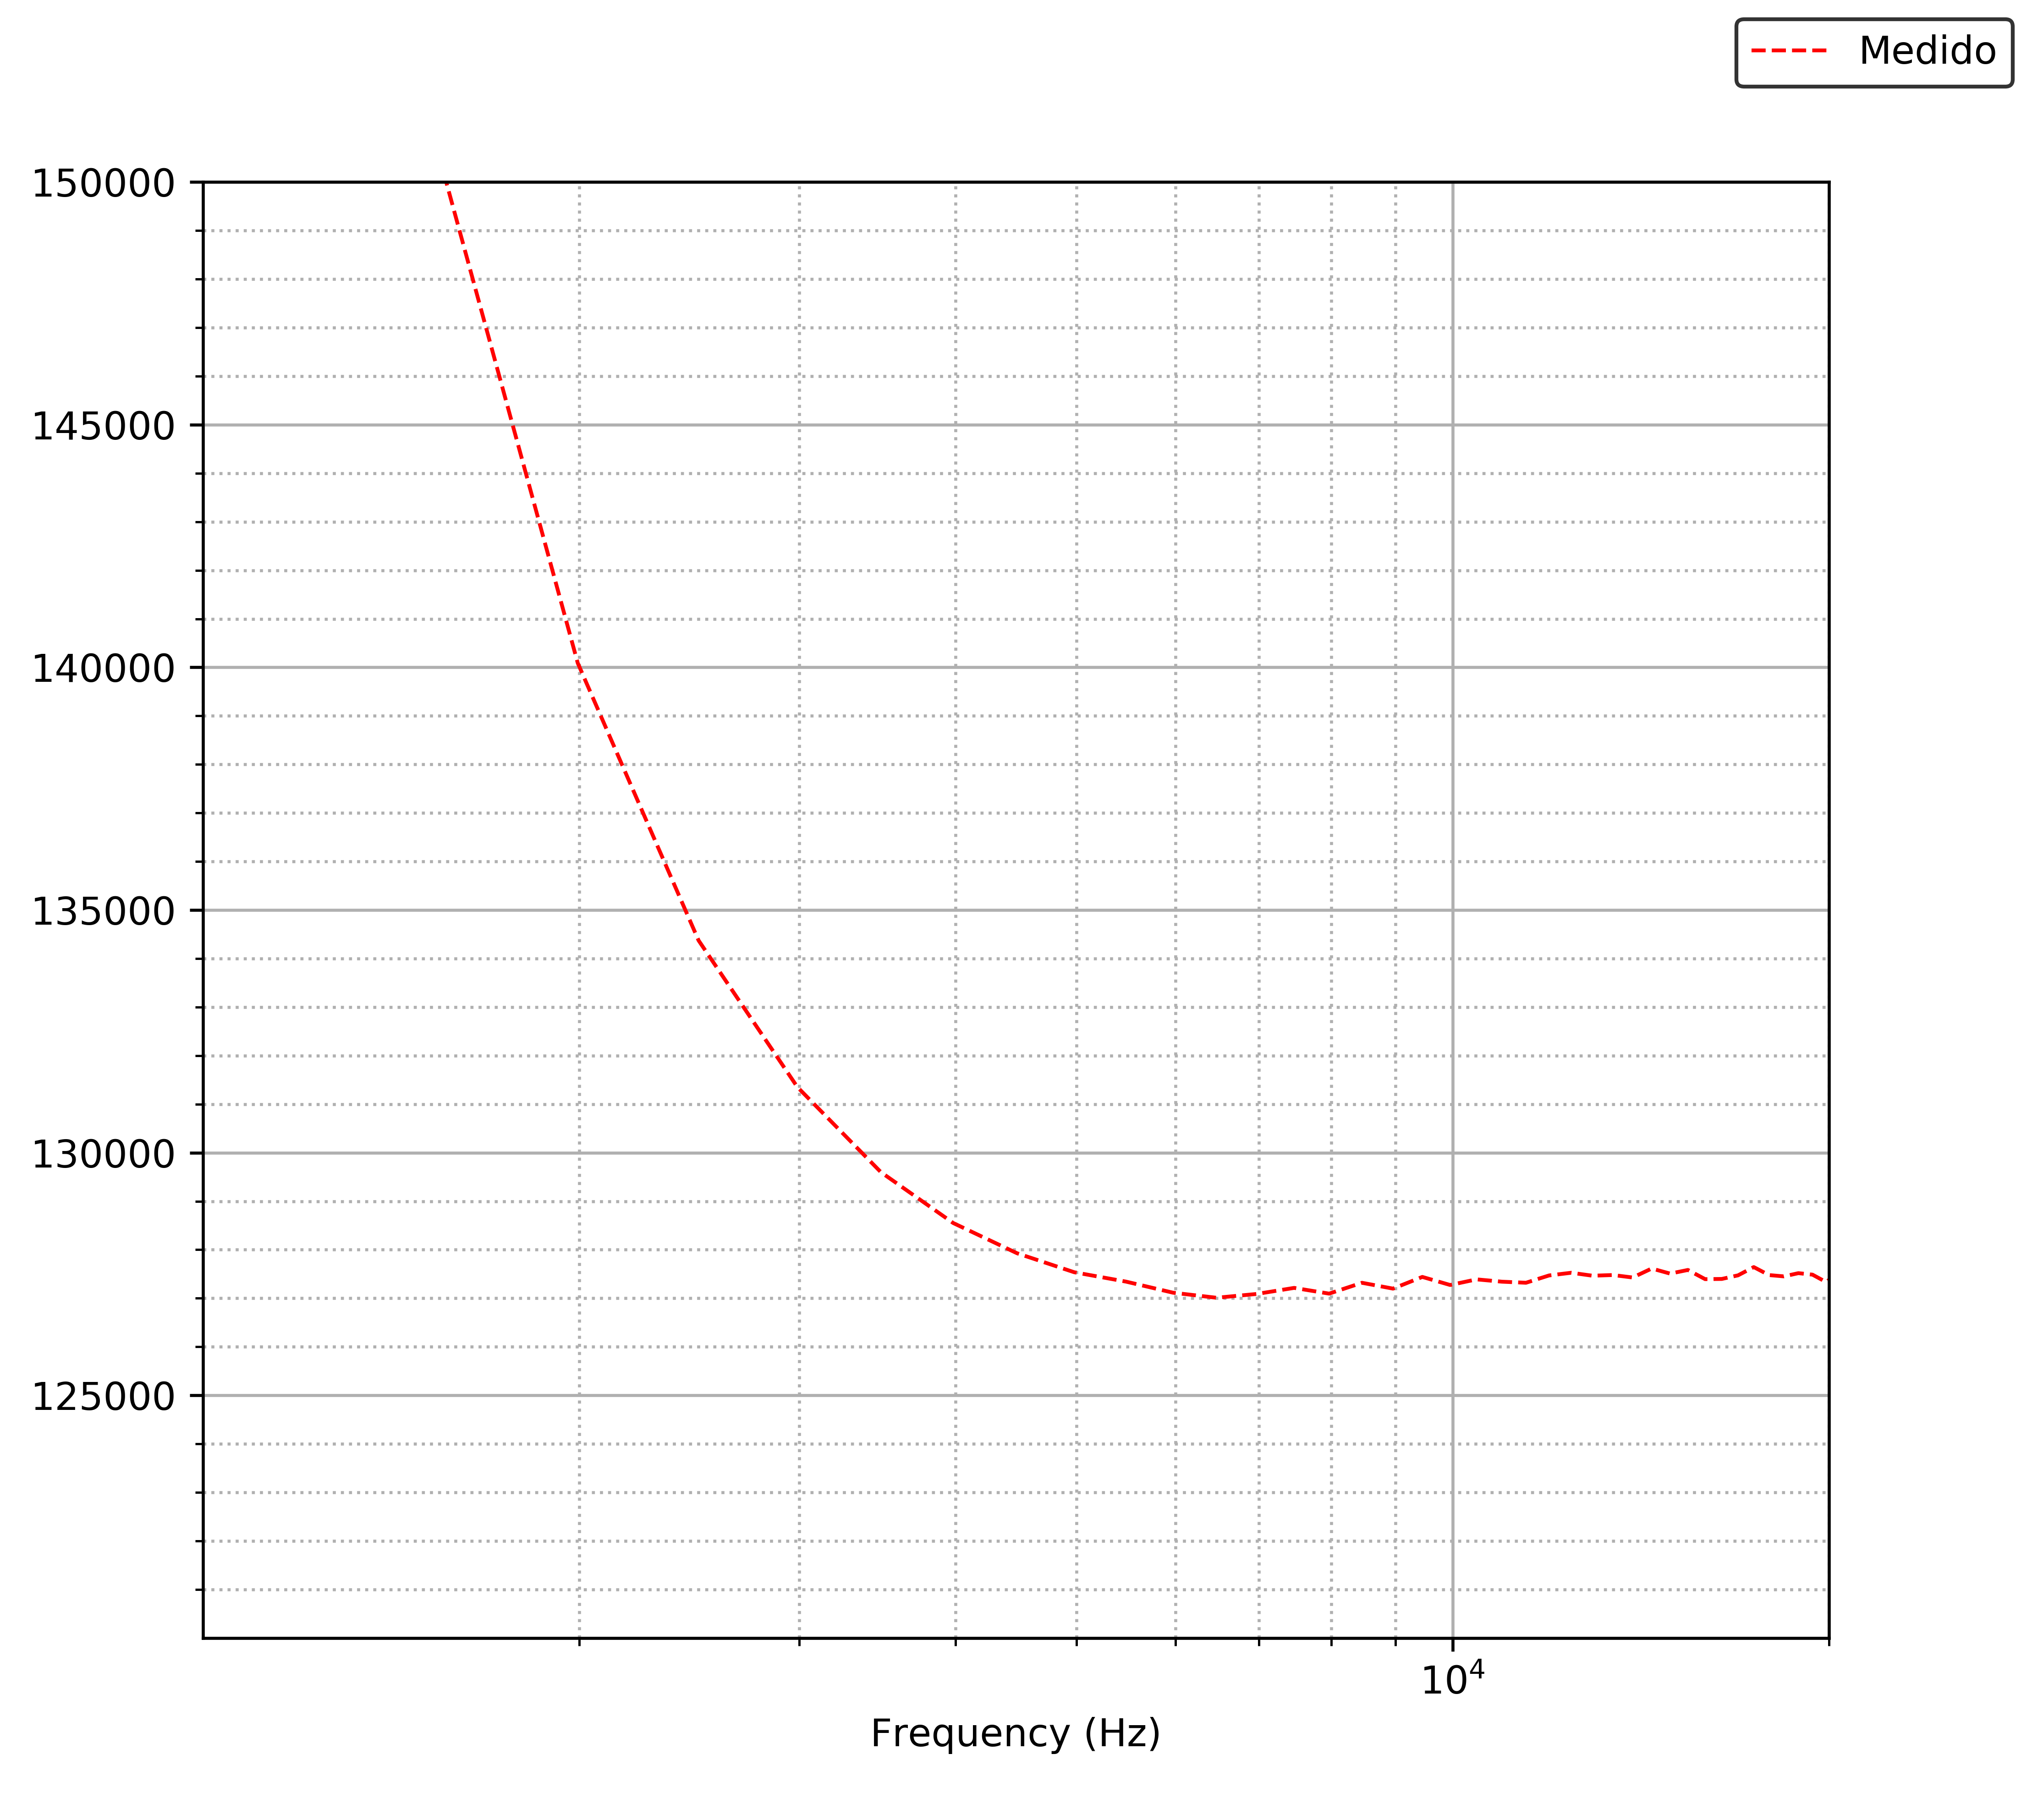
\includegraphics[scale=0.1]{../EJ1/Recursos/bessel_impedancia_entrada.png}
    \caption{Impedancia de entrada medida}
    \label{bessel_impedancia_entrada}
\end{figure}

\paragraph{Retardo de grupo:} En la Fig. \ref{fig:bessel_group_delay} se puede observar el retardo de grupo del filtro, contrastando tanto los resultados medidos como te\'oricos de la aproximaci\'on.
Es importante observar para la frecuencia $f_p = 550Hz$, efectivamente la desviaci\'on es menor al $5\%$ tal cual fue consignado..

\begin{figure}[H]
    \centering
    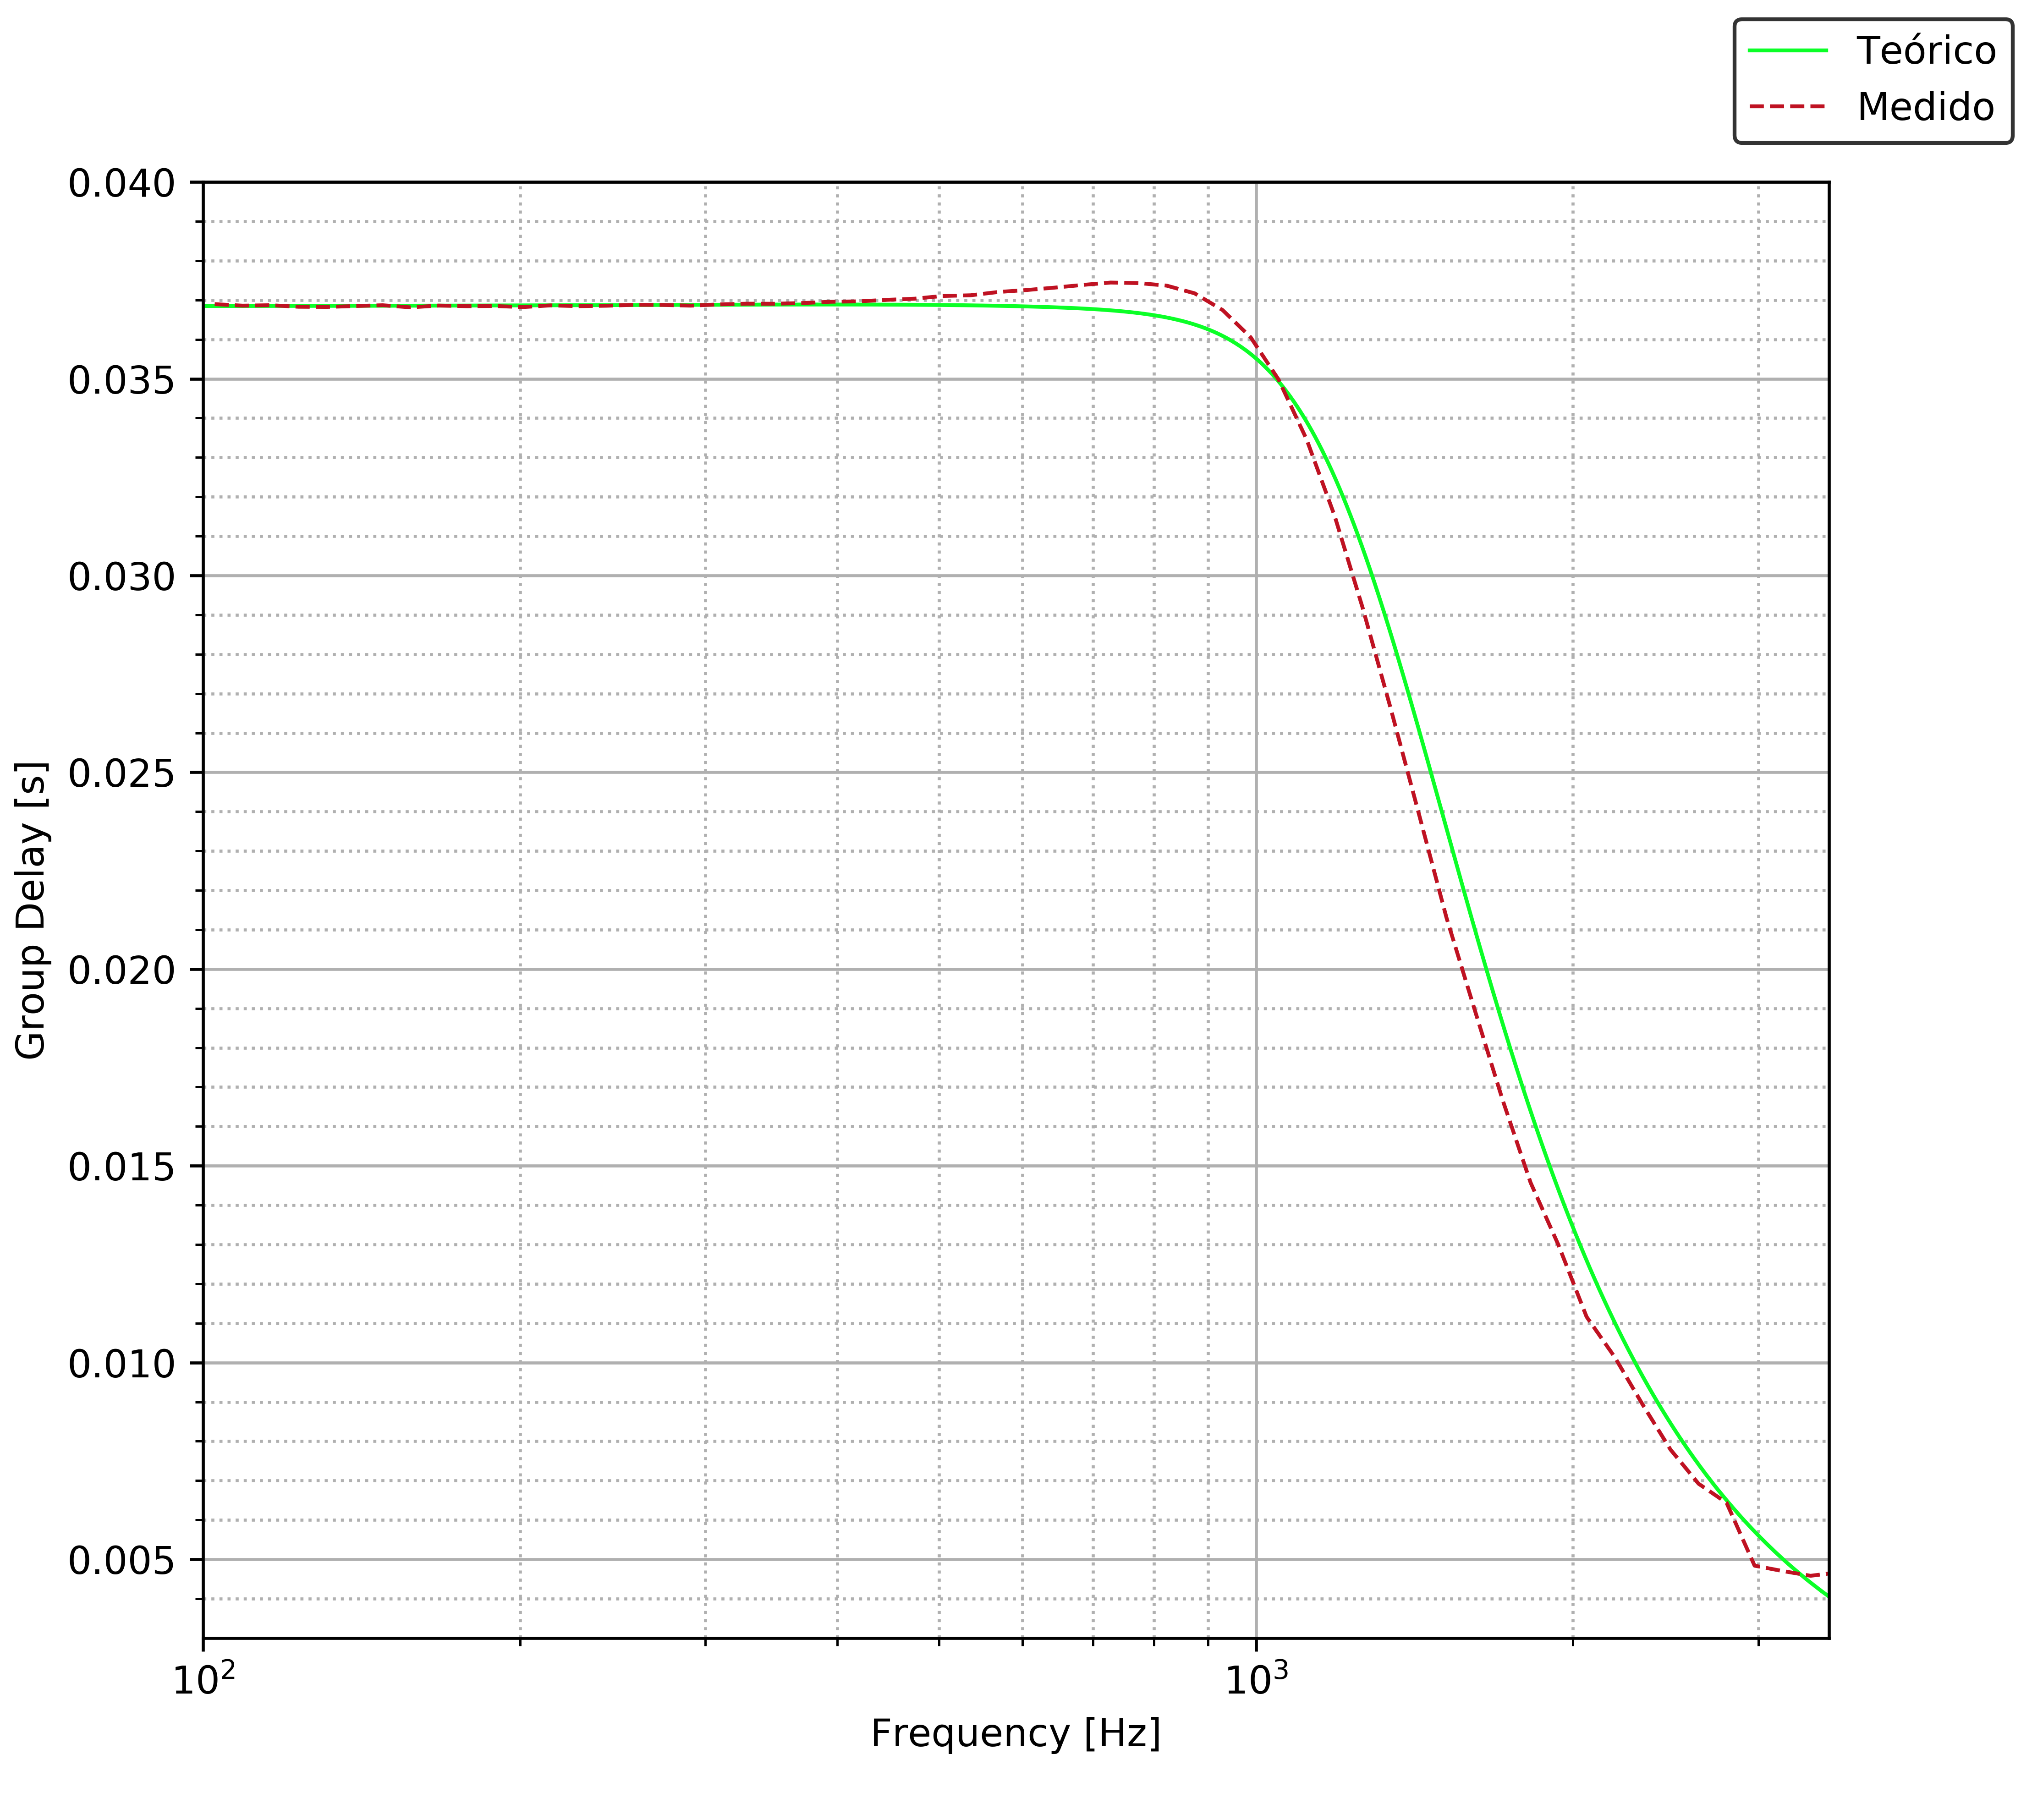
\includegraphics[scale=0.7]{../EJ1/Recursos/bessel_group_delay.png}
    \caption{Retardo de grupo de Bessel}
    \label{fig:bessel_group_delay}
\end{figure}

\subsection{Dise\~no de PCB}
En la pr\'actico se reutiliz\'o el mismo dise\~no de PCB para ambos filtros, empleando una configuraci\'on de entrada Sallen Key,
que sin conectar el capacitor de la realimentaci\'on se convierte en un filtro de primer orden RC con buffer, lo necesario para el caso
de Legendre. Se pueden visualizar los resultados de PCB en la Fig. \ref{fig:pcb_altium_3d}.

\begin{figure}[H]
    \centering
    \begin{tabular}{c c}
        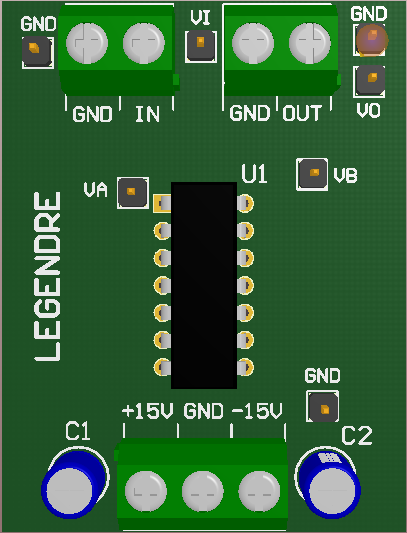
\includegraphics[scale=0.5]{../EJ1/Recursos/legendre_top_3d.PNG} & 
        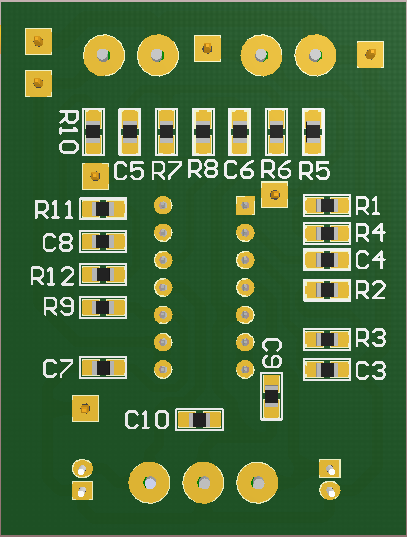
\includegraphics[scale=0.5]{../EJ1/Recursos/legendre_bottom_3d.PNG} \\
        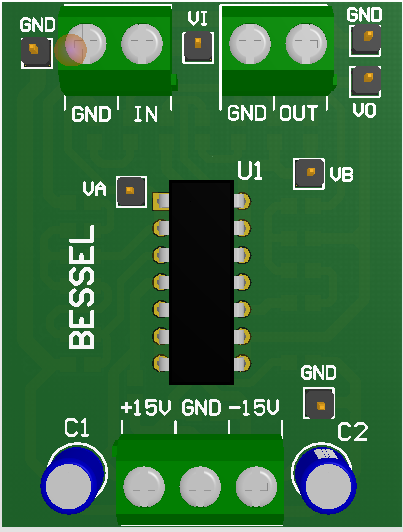
\includegraphics[scale=0.5]{../EJ1/Recursos/bessel_top_3d.PNG} & 
        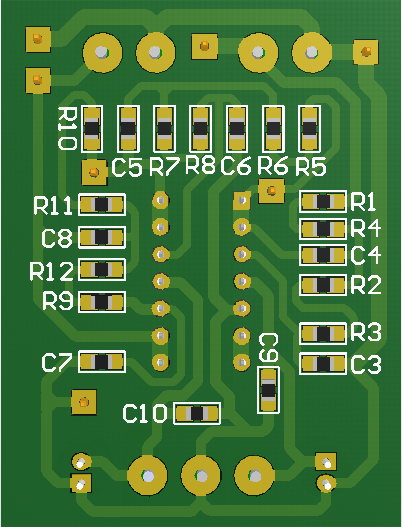
\includegraphics[scale=0.5]{../EJ1/Recursos/bessel_bottom_3d.PNG}
    \end{tabular}
    \caption{Dise\~nos de PCB en Altium Designer}
    \label{fig:pcb_altium_3d}
\end{figure}

\subsection{Conclusiones}
Las celdas de Sallen Key son \'utiles para implementar funciones de aproximaci\'on de segundo orden con muy baja sensibilidad, garantizando que ante plantillas un poco m\'as restrictivas, las variaciones
pr\'acticas sean casi imperceptibles, sin necesidad de mayor ajuste que la definici\'on de los componentes a tolerancias del $1\%$ o al $10\%$ seg\'un el caso. Por otro lado, est\'a limitada a trabajar con valores
bajos de factor de calidad, evitando utilizar mucha ganancia para no inestabilizar al sistema. En conclusi\'on, se recomienda el uso de esta celdas para aquellas etapas de bajo factor de calidad y ganancia moderada siempre
que sea posible.
